% !TEX program = xelatex
\documentclass{InforMeX}

\begin{document}
\sloppy
\portada{Máster en Ingeniería de Sistemas y Control}
{Optimización Heurística y Aplicaciones}
{Javier Arambarri Calvo}
{2025/2026}
{\today}
{Proyecto: optimización del \textit{rendezvous} para dos \textit{cobots}
cooperativos}

%%%%%%%%%%%%%%%%%%%%
% \datos{1}{2}{3}
%  1- color -> imprime logo en color; cc-> imprime logo en B/N
%  2- Título del documento
%  3- Nombre del Vicerrectorado
%%%%%%%%%%%%%%%%%%%%
\include{autoria}

\renewcommand{\tablename}{Tabla}
%\renewcommand{\listtablename}{Índice de tablas}


\datos{color}{}{}
\tableofcontents
%\newpage
%\listoffigures
%\newpage
%\listoftables
%\lstlistoflistings

\newpage
%%%%%%%%%%%%%%%%%%%%
% \adaptar{1}{2}
% 1- Si -> aumentar tamaño de letra
% 2- Si -> Adaptado con colores de Baja Visión
%%%%%%%%%%%%%%%%%%%%
\adaptar{no}{no}

\datos{color}{}{}
\section*{Introducción}
\addcontentsline{toc}{section}{Introducción}

Esta memoria recoge el trabajo realizado en la asignatura de Optimización Heurística y Aplicaciones 
del Máster en Ingeniería de Sistemas y de Control. \\

A lo largo de la asignatura se han ido recibiendo correcciones por parte del equipo docente 
que se han subsanado.\\

Asimismo, en el caso de la implementación de la técnica de búsqueda
local se han identificado diversas dificultades que han requerido la modificación
de la definición del problema. Por ello, estas modificaciones se han ido comentando según se
resolvía el problema y se ha mantenido la versión inicial en las secciones correspondientes
con el fin de reflejar la evolución sufrida. \\

Este documento se organiza de la siguiente manera: en la sección Tarea se 
describe la tarea de la asignatura, en la sección de la Propuesta
se define la problemática a resolver, en la sección de la Propuesta Técnica
de Búsqueda Local se presenta la propuesta inicial realizada en el tema 2 y 
por último, en la sección de Revisión y Desarrollo de la Propuesta Técnica de Búsqueda
Local se actualiza la propuesta inicial, se aplican las modificaciones oportunas
para conseguir resolver el problema y se exponen los resultados obtenidos.
\datos{color}{}{}
\section*{Tarea}
\addcontentsline{toc}{section}{Tarea}
%\addcontentsline{toc}{section}{Ejercicio 1}
Como uno de los objetivos fundamentales de la asignatura es conseguir que los
alumnos sean capaces de enfrentarse a un problema de optimización real con 
las técnicas aprendidas, el primer trabajo que se propone consiste en que 
cada alumno sugiera el problema de optimización que desee resolver a lo largo
de la asignatura, identifique sus variables de decisión, funciones objetivo,
restricciones, grupo al que pertenecen, etc. \\

Con el objeto de nivelar los problemas elegidos por los alumnos, 
los problemas elegidos serán propuestos por los alumnos a los
profesores de la asignatura, y analizados, modificados, refinados,
y finalmente aceptados o rechazados por los últimos hasta
alcanzar una propuesta formal del problema que los alumnos irán resolviendo
a lo largo de la asignatura. \\

Este proceso de definición y selección de problemas se realizará durante el estudio de los contenidos de este primer tema.
Debido al trabajo en equipo que se establece entre los profesores y los alumnos, se proponen dos fechas finales de entrega de
la definición del problema:

\begin{itemize}
    \item 15 de Marzo: Fecha limite de entrega de la propuesta inicial del problema en la que el alumno presentará un documento que
describa (cualitativamente) las características mas relevantes del problema que desea resolver, identificando las variables de
decisión y las funciones de mérito utilizadas para medir los objetivos y restricciones del problema.

    \item Durante las dos semanas sucesivas, los profesores y el alumno analizaran el problema, lo modificarán, etc... con el objeto
de acordar una propuesta inicial definitiva antes del 29 de Marzo. Para esta fecha, el alumno documentará la propuesta
definitiva a los profesores, poniendo de manifiesto las variables de decisión, funciones de merito, restricciones, clasifi-
cación del problema, etc... Además, implementará las funciones responsables de medir la bondad (mérito y restricciones)
de una posible solución del problema. En las sesiones de dudas del tema (Semana 23 - 27 Febrero) se propondrá a
los alumnos la cabecera de la función, de forma que sea utilizada, sin cambios significativos, durante los siguientes temas.
\end{itemize}
\datos{color}{}{}
\section*{Propuesta: optimización del \textit{rendezvous} para dos \textit{cobots} cooperativos}
\addcontentsline{toc}{section}{Propuesta: optimización del \textit{rendezvous} para dos \textit{cobots} cooperativos}

En el grupo de investigación en el que trabajo estamos comenzando un 
proyecto enmarcado en la agricultura vertical. En este sentido, estamos 
preparando un entorno, tanto real como simulado (Figura \ref{fig:sim}),
en el que dos robot manipuladores colaborativos van a desempeñar diferentes
tareas. Debido a que todavía estamos definiendo el escenario, lo más 
probable es que este varíe respecto de la imagen presentada, aunque
esas modificaciones no serán estructurales. Dos de los cambios incluyen 
que el robot de la izquierda tendrá también sus propias estanterías y que el 
robot de la derecha trabajará cerca 
de la pared cuando el eje lineal de desplazamiento sobre el que se coloca
esté en uno de sus extremos. \\

\begin{figure}[H]
  \centering
  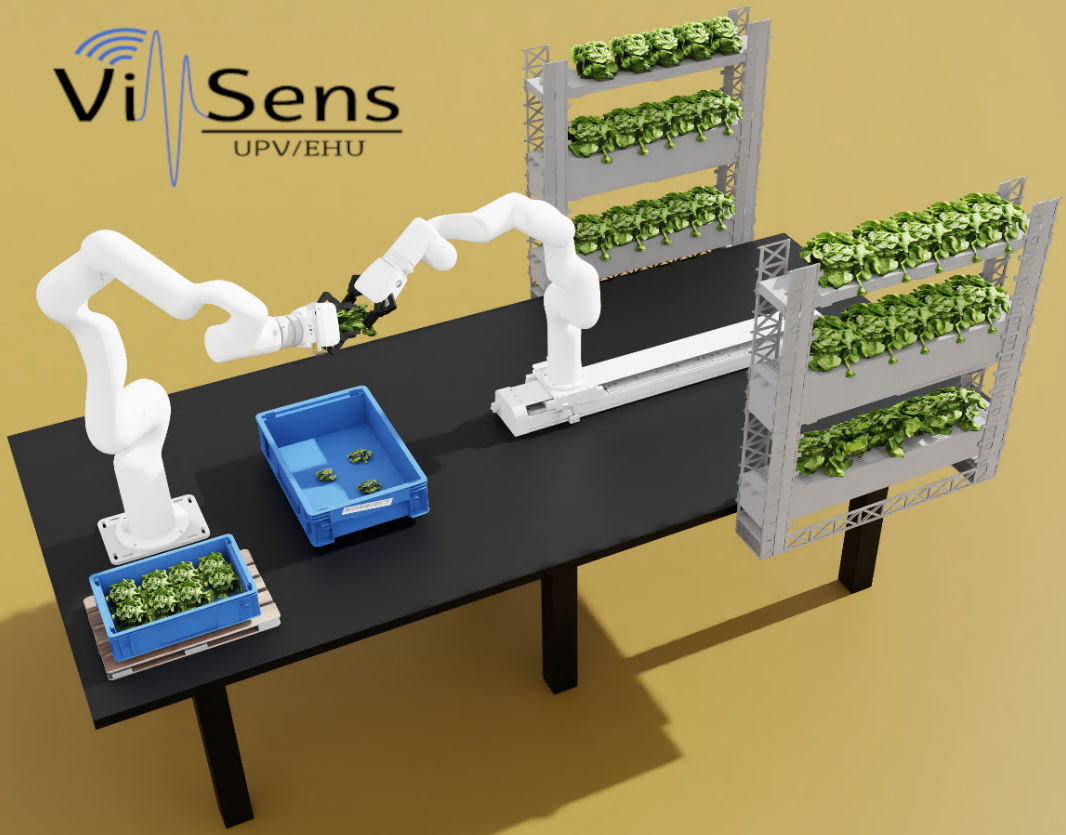
\includegraphics[scale=0.25]{Images/escenario3_visens.png}
  \caption{Escenario simulado.}
  \label{fig:sim}
\end{figure}

Este escenario está compuesto por una mesa, dos robots manipuladores 
colaborativos y estanterías de cultivo y almacenaje. La mesa es la superficie
sobre la que se desarrollará toda la actividad, por lo que los robots 
no deben exceder sus límites. El primer robot, el \textit{UFactory 850} \cite{ufactory_xarm850}, 
es el que está colocado a la izquierda en la Figura \ref{fig:sim}, y está
fijo a la mesa. El segundo robot, el \textit{UFactory xArm6} \cite{ufactory_xarm850}, es el que 
se encuentra a la derecha en la Figura \ref{fig:sim}, y está montado sobre un eje 
lineal de desplazamiento que le permite aumentar su espacio de trabajo.
Ambos robots están equipados con pinza, cámara de visión y sensor de fuerza 
en el efector. Las estanterías correspondientes a cada robot están colocadas de manera que son completamente 
alcanzables por los dos manipuladores. \\

El segundo robot se encargará de supervisar el estado de los cultivos o 
aplicarles alguna operación, 
y cuando considere necesario (bien sea por visión, o por tiempo de cultivo, por ejemplo)
retirará un cultivo para realizarle una operación o tratamiento que necesite 
de la cooperación con el primer robot, por ejemplo, la retirada de hojas enfermas.
En función del tratamiento aplicado, la hortaliza deberá volver a su 
estantería de cultivo, mediante el segundo robot, o ir a la estantería de almacenaje. 
En caso de ser almacenada,
será el primer robot el encargado de ejecutar dicha tarea. 
Por su parte, el primer robot traslada las hortalizas 
de la estantería de almacenaje a un palet o realiza alguna operación específica 
sobre las plantas en este momento del cultivo.\\

Además, en las tareas cooperativas será preciso controlar la fuerza aplicada 
por cada robot para evitar dañar las hortalizas, que se caracterizan 
por ser deformables. Siempre y cuando esta fuerza se controle adecuadamente 
por ambos robots, el punto de cooperación de los robots no tiene 
por qué ser fijo, esto es, en función de la situación instantánea de 
cada robot ese punto podrá darse en diferentes coordenadas, pero 
siempre garantizando que la fuerza aplicada a la planta es la adecuada. \\

%No obstante, por simplicidad este control de fuerzas podría quedar 
%fuera del problema de optimización. \\

Con todo ello, se busca un sistema autónomo y adaptativo en el que
los dos robots decidan en cada instante qué operación ejecutar
—retirar hojas, realizar tratamientos, regar, germinar o mover 
plantas al almacén, por ejemplo— de modo que el conjunto minimice el tiempo de
ciclo, o, en otras palabras, maximice la eficiencia operativa. \\

Como se ha explicado, este sistema está compuesto de múltiples partes,
pero esta propuesta de problema de optimización se va a centrar en el punto 
espacial de cooperación. A este punto se le denomina \textit{rendezvous}. 

\section*{Objetivo}
Obtener las posiciones, \(\mathbf{p}_r=(x_r,y_r,z_r)\), y orientaciones,
\(\mathbf{q}_r=(q_{r_0},q_{r_1},q_{r_2},q_{r_3})\), de los efectores de cada robot,
$r\in\{A,B\}$,
y los 
factores de velocidad de ejecución de movimiento de cada robot, \(\mathbf{s}_r\), incluyendo el 
del eje lineal de desplazamiento \(\mathbf{s}_{rail}\), que permitan
sincronizar la llegada de ambos robots al \textit{rendezvous} óptimo calculado ($p_r,\,q_r$) 
sincronizando y minimizando el 
tiempo de desplazamiento necesario, $t_{r}(\mathbf{p}_r,\mathbf{q}_r,\mathbf{s}_r)$,
según el estado actual de cada robot (posición actual). \\

Las posiciones se definen en el espacio de la tarea de cada robot y en metros, las 
orientaciones en cuaterniones, los factores de 
velocidad podrán tomar cualquier valor entre 0 y 1, y el tiempo de desplazamiento
se mide en segundos. La elección de cuaterniones para representar la orientación no es trivial,
dado que es la fórmula computacionalmente más 
eficiente \cite{barrientos2007fundamentos} al no presentar singularidades, ser más compactos y 
fáciles de normalizar.\\

Por tanto, se buscan las posiciones y orientaciones de los efectores 
\(\mathbf{p}_A=(x_A,y_A,z_A)\), \(\mathbf{p}_B=(x_B,y_B,z_B)\), 
\(\mathbf{q}_A=(q_{A_0},q_{A_1},q_{A_2},q_{A_3}),\, \mathbf{q}_B=(q_{B_0},q_{B_1},q_{B_2},q_{B_3})\), y los factores de velocidad de cada robot 
\(\mathbf{s}_A,\, \mathbf{s}_B,\, \mathbf{s}_{rail}\), tal que minimicen 
el tiempo de desplazamiento de cada robot al punto de cooperación,
$t_A(\mathbf{p}_A,\mathbf{q}_A,\mathbf{s}_A)$ y $\,t_B(\mathbf{p}_B,\mathbf{q}_B,\mathbf{s}_B,\mathbf{s}_{rail})$, 
y ambos sean lo más parecidos posible. \\

Es decir, ambos robots deben llegar sincronizados al \textit{rendezvous}.Es importante mencionar que,
puesto que el segundo robot $B$ está sobre un eje lineal de desplazamiento, su tiempo $t_B$ tiene que
tener en cuenta también el factor de velocidad de dicho eje, $s_{rail}$. \\

En el punto de cooperación o \textit{rendezvous} los efectores deben quedar enfrentados,
esto es, alineados en dos ejes del mundo y separados por una determinada distancia en el otro. 
Esta configuración, Figura \ref{fig:conf}, implica que la diferencia en la orientación
en ambos será de 180º y la distancia se medirá en línea recta desde los orígenes
de ambos efectores, para lo que será necesario convertir las posiciones $p_A$ y $p_B$
a coordenadas del mundo.

\begin{figure}[H]
  \centering
  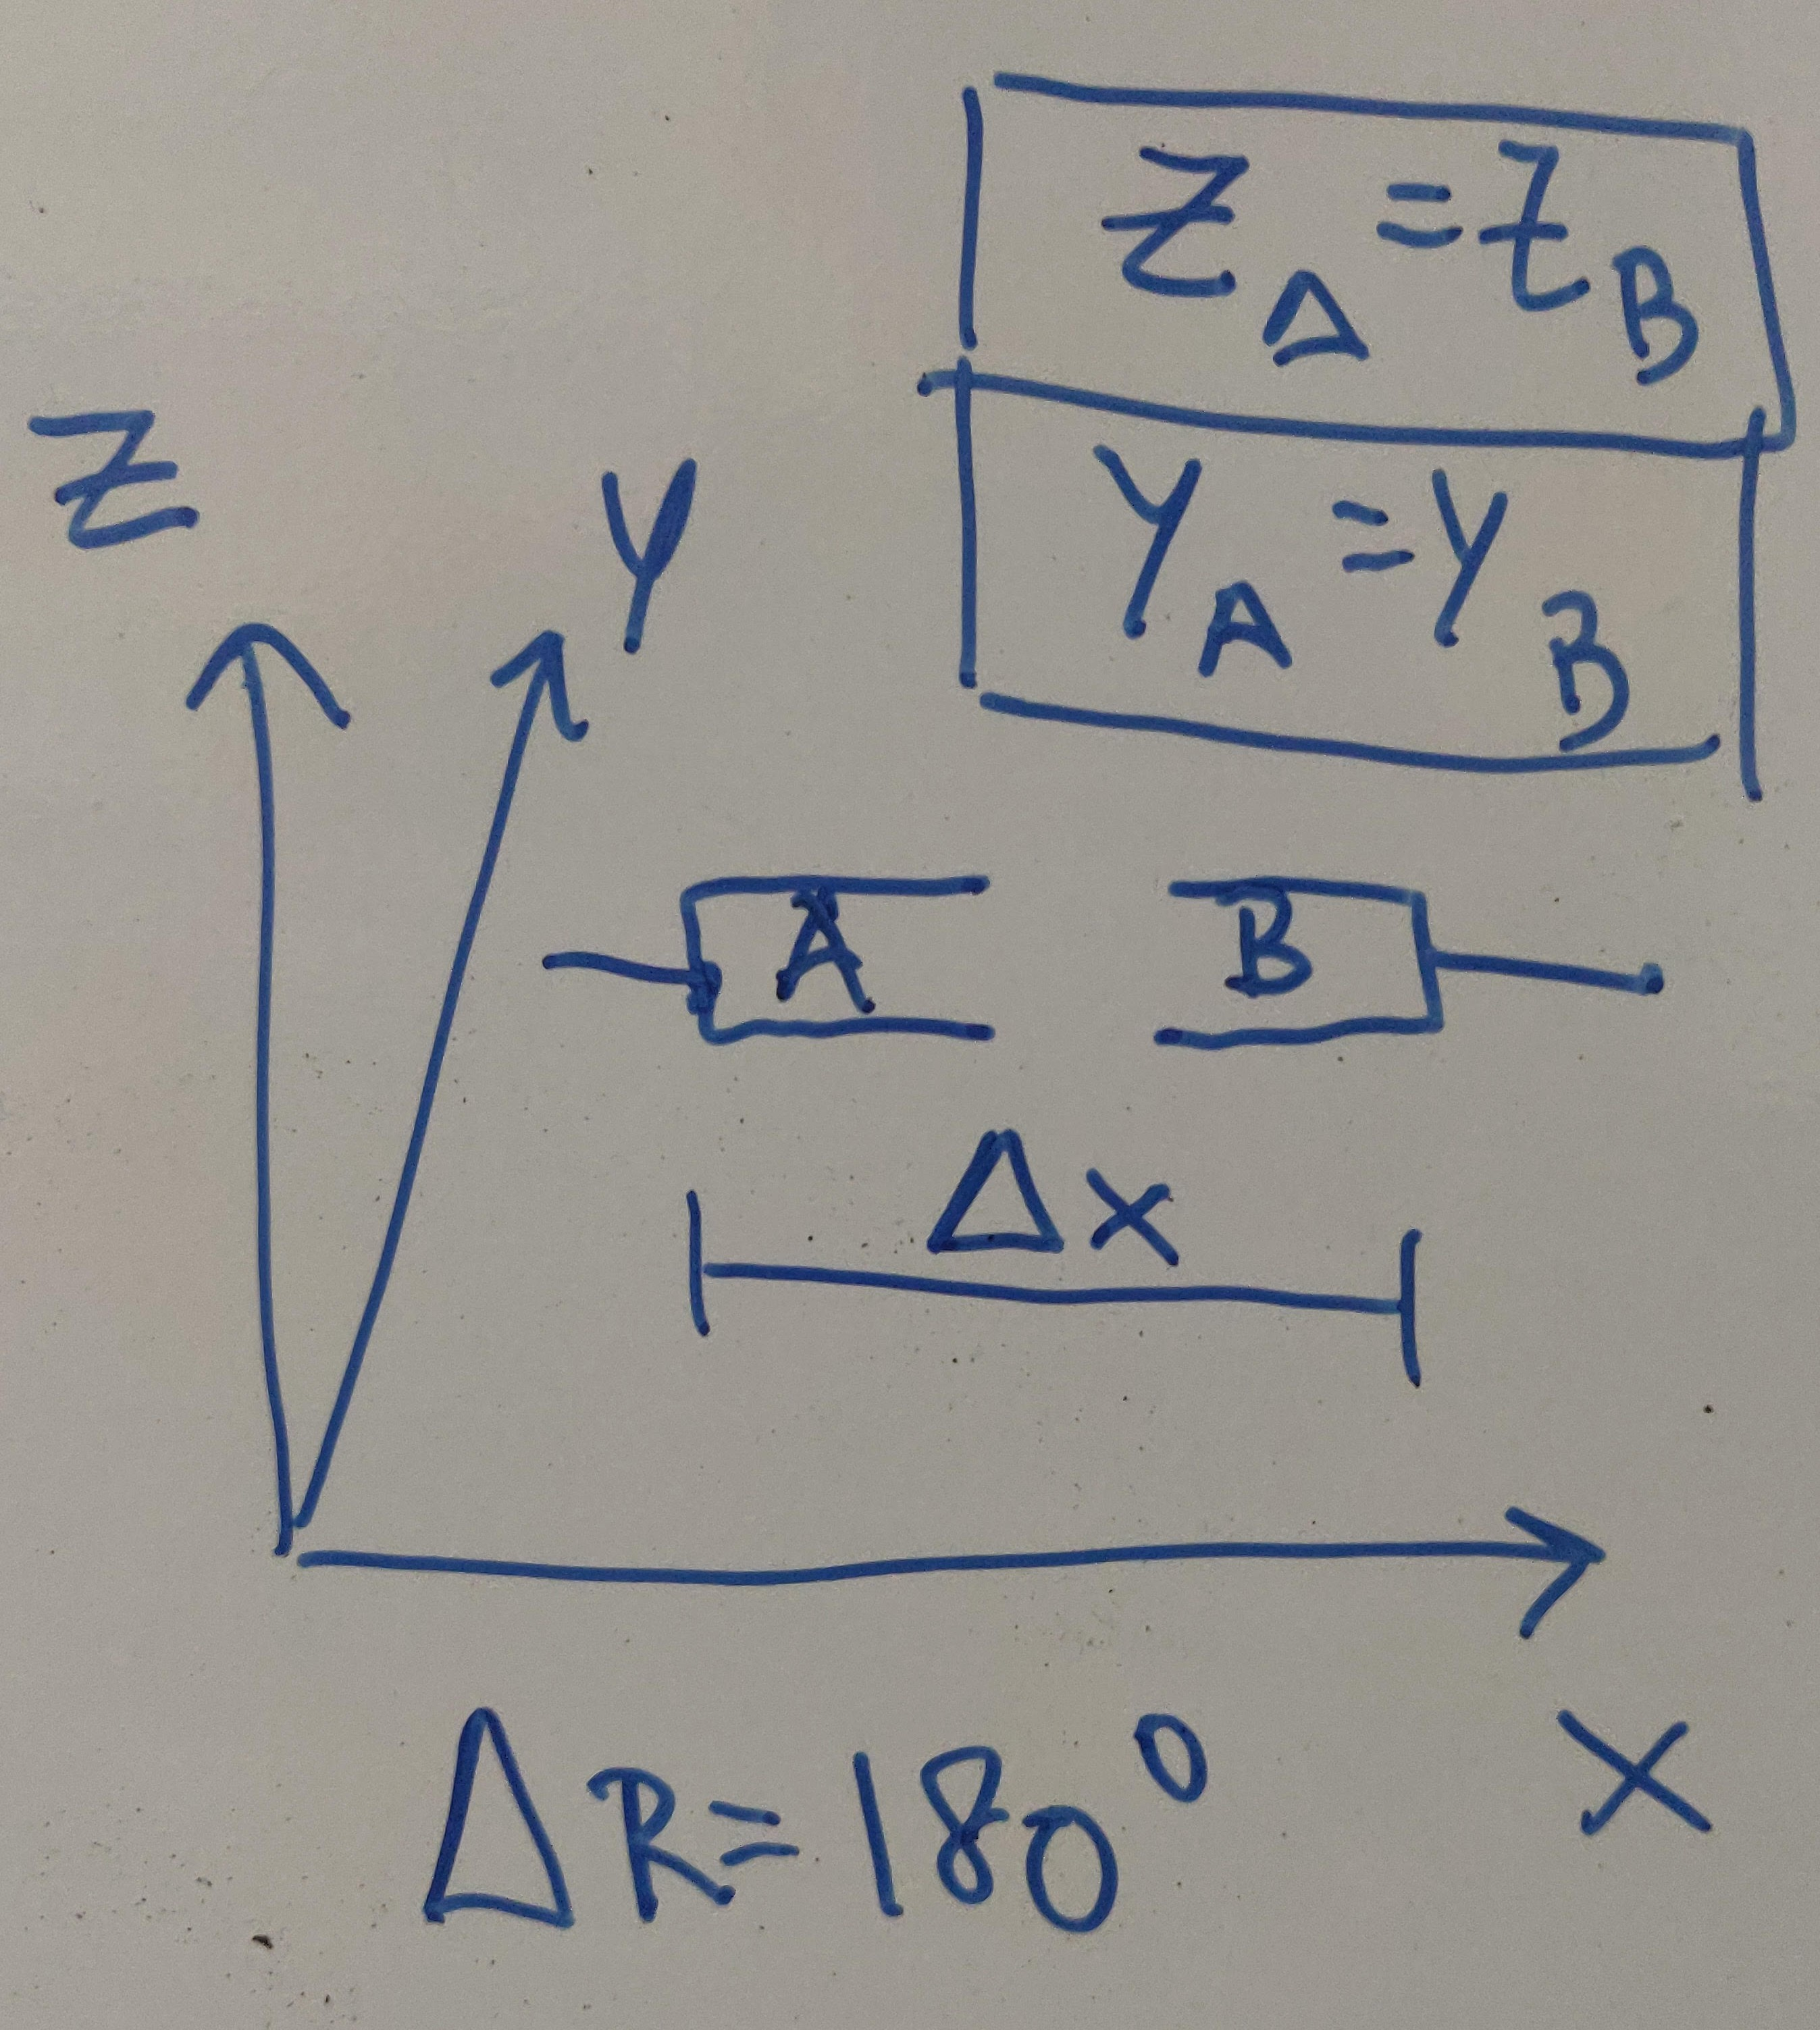
\includegraphics[scale=0.05]{Images/ejemplo.jpg}
  \caption{Croquis de la configuración propuesta.}
  \label{fig:conf}
\end{figure}

En otras palabras, el objetivo es obtener las coordenadas óptimas del punto de cooperación \textit{rendezvous}
y los factores de velocidad de cada robot de manera que se minimice el tiempo de llegada 
sincronizada al mismo.


\section*{Variables de decisión}
\addcontentsline{toc}{subsection}{Variables de decisión}
Se tiene un total de 17 variables de decisión:
\begin{itemize}
  \item \textbf{Posiciones objetivo de efectores}: \(\mathbf{p}_A=(x_A,y_A,z_A)\), \(\mathbf{p}_B=(x_B,y_B,z_B)\) 
  en el espacio de la tarea de cada robot.
  \item \textbf{Orientaciones objetivo de efectores}: 
  \(\mathbf{q}_A,\, \mathbf{q}_B \in S^3,\) donde cada cuaternión unitario $\mathbf{q}=(q_{0},q_{1},q_{2},q_{3})$ representa una rotación en $SO(3)$.
  %\(\mathbf{R}_A,\mathbf{R}_B\in SO(3)\).
  \item \textbf{Escalas de velocidad}: \(\mathbf{s}_A,\mathbf{s}_B, \mathbf{s}_{rail}\in(0,1]\).
\end{itemize}

\begin{comment}
\subsection*{Parámetros y variables derivadas}
\addcontentsline{toc}{subsection}{Parámetros y variables derivadas}

\begin{itemize}
  \item \textbf{Variables derivadas}: \(t_A,t_B\) tiempos estimados de llegada, calculados mediante la función de tiempo
  

\[
  t_r(\mathbf{p}_r,\mathbf{R}_r,s_r),
  \]


  y no tratadas como variables independientes en la optimización.
  \item \textbf{Parámetros del problema}: \(d_{\text{ef}}\) (distancia objetivo entre efectores), \(\text{eje}\in\{x,y\}\) (eje del mundo para la separación), \(\epsilon\) (tolerancia posicional), \(\Delta t_{\max}\) (tolerancia temporal de sincronización), \(s_{\min}\), \(m_{\min}\), y otros límites físicos.
\end{itemize}
\end{comment}

\section*{Función objetivo}
\addcontentsline{toc}{subsection}{Función objetivo}
\[
\min_{\mathbf{p}_A,\mathbf{q}_A,\mathbf{p}_B,\mathbf{q}_B,\mathbf{s}_A,\mathbf{s}_B,\mathbf{s}_{rail}}\; 
T_{\text{rendezvous}} \;=\; \min\; \max\big(t_A(\mathbf{p}_A,\mathbf{q}_A,\mathbf{s}_A),\,t_B(\mathbf{p}_B,\mathbf{q}_B,\mathbf{s}_B,\mathbf{s}_{rail})\big),
\]

donde los tiempos $t_A$ y $t_B$ se refiere a los tiempos $t_{r}(\mathbf{p}_r,\mathbf{q}_r,\mathbf{s}_r)$
necesarios por cada robot para alcanzar
el punto de cooperación. Se estima de la siguiente manera:
\[
t_{r}(\mathbf{p}_r,\mathbf{q}_r,\mathbf{s}_r)
=\frac{\text{dist\_rail}(\mathbf{p}_r)}{s_{rail}\,v_{\text{rail}}}
+\frac{\ell_r(\mathbf{p}_r,\mathbf{q}_r)}{s_r\,v_{\text{arm},r}},
\]

%donde \(\ell_r\) aproxima la distancia efectiva necesaria para alcanzar posición y orientación.\\

En esta expresión \(\mathrm{dist\_rail}(\mathbf{p}_r)\) es la distancia a recorrer 
por el motor lineal (raíl) en metros (si no existe raíl, es decir, el robot 
está fijo -robot A-, se toma \(0\)),
\(v_{\text{rail}}\) es la velocidad del raíl en \(\mathrm{m/s}\), 
\(\ell_r(\mathbf{p}_r,\mathbf{R}_r)\) es la longitud
efectiva del movimiento del brazo en metros (por ejemplo, la distancia euclídea del efector
desde su posición inicial con todas las articulaciones en posición $0$), y \(v_{\text{arm},r}\) es la 
velocidad del brazo en \(\mathrm{m/s}\). Dividir por \(s_r\)
reduce la velocidad efectiva y por tanto, aumenta el tiempo. \\

Cabe mencionar que la primera evaluación del equipo docente valoró la sustitución de la función
$\min\; \max (·)$ por un frente de pareto multiobjetivo con dos funciones objetivo, una por cada robot:

\[
\min_{\mathbf{p}_A,\mathbf{q}_A,\mathbf{p}_B,\mathbf{q}_B,\mathbf{s}_A,\mathbf{s}_B,\mathbf{s}_{rail}}
\;\; \mathbf{T}(\cdot),
\]

con
\[
\mathbf{T}(\cdot) = 
\begin{bmatrix}
t_A(\mathbf{p}_A,\mathbf{q}_A,\mathbf{s}_A) \\
t_B(\mathbf{p}_B,\mathbf{q}_B,\mathbf{s}_B,\mathbf{s}_{rail})
\end{bmatrix},
\]

Así, una solución $\mathbf{x}^\star$ se considera óptima en el sentido de Pareto si no 
existe otra solución factible $\mathbf{x}$ tal que
\[
t_A(\mathbf{x}) \le t_A(\mathbf{x}^\star), \qquad
t_B(\mathbf{x}) \le t_B(\mathbf{x}^\star),
\]

y al menos una de las desigualdades sea estricta ($<$). El conjunto de todas las soluciones 
Pareto-óptimas constituye el frente de Pareto en el plano $(t_A,t_B)$, que describe 
los compromisos entre minimizar el tiempo de llegada del robot A y el del robot B. \\

Mientras que con Pareto no hay una única solución y se necesitaría
un criterio externo para elegir un punto de entre los Pareto-óptimos,
la formulación con $\min\; \max (·)$ obtiene una única solución. Puesto que se 
desea que ambos robots lleguen sincronizados, en otras palabras, que tarden lo mismo, 
se va a optar por $\min\; \max (·)$, aunque se deja la puerta abierta a 
resolver también el problema como frente de Pareto y así desarrollar una comparativa.


\section*{Restricciones}
\addcontentsline{toc}{subsection}{Restricciones}
\begin{itemize}
  \item Separación final en coordenadas del mundo. Los efectores deben quedar separados 
  por la distancia objetivo \(d_{\text{ef}}\) en el eje asignado, cuyo eje unitario se representa mediante 
  $\mathbf{e}_{\text{eje}}^\top$, y con tolerancia \(\epsilon_{\text{eje}}\):
  $
  \big|\mathbf{e}_{\text{eje}}^\top\big((\mathbf{p}_A)-(\mathbf{p}_B)\big)-d_{\text{ef}}\big|\le\epsilon_{\text{eje}}
  $.

  \item Posición y orientación de enfrentamiento: \textit{rendezvous} enfrentado. 
  Siguiendo la representación de la Figura \ref{fig:conf}:\\
  \[\big|\mathbf{e}_{\text{Z}}^\top\big((\mathbf{p}_A)-(\mathbf{p}_B)\big)|\le\epsilon_Z, 
  \qquad\big|\mathbf{e}_{\text{Y}}^\top\big((\mathbf{p}_A)-(\mathbf{p}_B)\big)|\le\epsilon_Y\]
  \[
  \|\operatorname{Log}(\mathbf{R}_B \mathbf{R}_A^\top \mathbf{R}_{\pi}^\top)\|\le \epsilon_{\theta},
  \]

  %donde \(\mathbf{R}_{\pi}\) es la rotación de 180° que define la orientación volteada y \(\operatorname{Log}(\cdot)\)
  %es el mapa logaritmo de rotaciones (norma en radianes).
  %, que convierte una matriz de rotación
  %en su representación eje-ángulo, de modo que la norma del resultado mide directamente el
  %ángulo mínimo de rotación necesario para ir de una orientación a otra. 
  %Por eso se usa en la desigualdad, ya que cuantifica la desviación angular (en radianes) 
  %respecto a la orientación volteada (\url{https://cvg.cit.tum.de/_media/members/demmeln/nurlanov2021so3log.pdf},
  %\url{https://colab.research.google.com/github/borglab/gtsam/blob/develop/gtsam/geometry/doc/SO3.ipynb}). \\


  donde \(\mathbf{R}_{\pi}\) es la rotación de 180° que define la orientación volteada y \(\operatorname{Log}(\cdot)\)
  es el mapa logaritmo de rotaciones (norma en radianes). \\

  Aunque las orientaciones se parametrizan mediante cuaterniones en las variables de decisión, 
  para evaluar las restricciones resulta conveniente convertirlos a matrices de rotación $\mathbf{R}_r$. La 
  representación en $SO(3)$ permite operar directamente con la composición de rotaciones y, 
  en particular, aplicar el mapa logarítmico $\operatorname{Log}(\cdot)$, que transforma una 
  matriz de rotación en su representación eje–ángulo \cite{murray1994mathematical}. La norma de este vector proporciona una 
  medida angular interpretable y numéricamente estable del error entre orientaciones, equivalente
  al ángulo mínimo necesario para alinear una con la otra \cite{barfoot2014associating}. Por ello, la restricción 
  $\|\operatorname{Log}(\mathbf{R}_B \mathbf{R}_A^\top \mathbf{R}_{\pi}^\top)\|\le \epsilon_{\theta}$ 
  cuantifica de manera directa la desviación respecto a la orientación enfrentada deseada. De este
  modo, las restricciones de alineación y enfrentamiento pueden formularse de forma más natural y
  robusta, manteniendo al mismo tiempo la compacidad y suavidad de los cuaterniones como 
  parametrización principal en la optimización (\url{https://cvg.cit.tum.de/_media/members/demmeln/nurlanov2021so3log.pdf},
  \url{https://colab.research.google.com/github/borglab/gtsam/blob/develop/gtsam/geometry/doc/SO3.ipynb}). \\


  
  %Aunque las orientaciones se parametrizan mediante cuaterniones en las variables de decisión, 
  %para la formulación de las restricciones resulta conveniente convertirlos
  %a matrices de rotación. Esta representación en $SO(3)$ permite expresar de forma directa operaciones
  %geométricas como la composición de rotaciones, el cálculo del error relativo entre orientaciones o 
  %la aplicación del mapa logarítmico, cuya norma proporciona una medida angular interpretable y 
  %numéricamente estable. De este modo, las restricciones de enfrentamiento y alineación pueden 
  %formularse de manera más natural y robusta, manteniendo al mismo tiempo la compacidad y suavidad
  %de los cuaterniones como variables de decisión.

  Esta restricción, aparentemente dura, se ha diseñado como blanda puesto que el objetivo a largo
  plazo será que el \textit{rendezvous} se pueda alcanzar con diferentes orientaciones y alineaciones.
  No obstante, para simplificar el proyecto dentro de la asignatura, se instroduce la restricción.
  %Para formulaciones con cuaterniones:
  %\[
  %q_B \approx q_{\pi}\otimes q_A,\qquad
  %\arccos\big(|\langle q_B,\,q_{\pi}\otimes q_A\rangle|\big)\le \epsilon_{\theta}.
  %\]

  %Elige \(\epsilon_{\perp}\) pequeño (p. ej. \(10^{-3}\)) y \(\epsilon_{\theta}\) en radianes (p. ej. \(0.01\)–\(0.05\)) según tolerancias de la tarea.


%\[
%\mathbf{R}_B = \mathbf{R}_{\pi}\,\mathbf{R}_A
%\qquad\Longleftrightarrow\qquad
%\mathbf{R}_B\,\mathbf{R}_A^\top = \mathbf{R}_{\pi}.
%\]

%\[
%\mathbf{R}_B = \mathbf{R}_A\,\mathbf{R}_{\pi}^{\text{(tool)}},
%\]

%\[
%\mathbf{R}_{\pi}=\exp\big(\pi\,[\mathbf{u}]_\times\big)
%= I + 2\big(\mathbf{u}\mathbf{u}^\top - I\big),
%\]





  \item Sincronización temporal. Llegadas casi simultáneas dentro de la tolerancia \(\Delta t_{\max}\):
  $\big|t_A(\mathbf{p}_A,\mathbf{q}_A,\mathbf{s}_A)-t_B(\mathbf{p}_B,\mathbf{q}_B,\mathbf{s}_B,\mathbf{s}_{rail})\big| \le \Delta t_{\max}$.

  \item Límites de escala de velocidad: 
  $0 < s_A \le 1,\quad 0 < s_B \le 1,$
  siendo $1$ la velocidad máxima permitida por el robot. Esta restricción será por definición 
  del problema y no una restricción pura a validar por el algoritmo.

  \item Exclusión de singularidades y factibilidad cinemática.
  Para cada pose y orientación objetivo debe existir una solución de cinemática 
  inversa \(q_r\) alcanzable:

  $\exists q_r:\ FK_r(q_r)=(\mathbf{p}_r,\mathbf{R}_r),\qquad
  \sigma_{\min}\big(J_r(q_r)\big)\ge m_{\min}$,
  donde $\sigma_{\min}\big(J_r(q_r)\big)$ es el menor valor singular de la jacobiana en 
  $q_r$, es decir, una medida numérica de cuán cerca está la configuración de una singularidad.
  Valores pequeños indican pérdida de grado de libertad efectivo, es decir, que se 
  encuentra cerca de una singularidad. Si existen múltiples soluciones \textit{IK}
  (cinemática inversa), se selecciona la que maximice \(\sigma_{\min}\).

  \item Espacio de trabajo $\mathcal{W}_r$ y zonas prohibidas $\mathcal{Z}_{r}$ de 
  cada robot $r$.
  Las poses deben pertenecer al espacio de trabajo y evitar zonas prohibidas:
  $
  (\mathbf{p}_r,\mathbf{R}_r)\in\mathcal{W}_r\setminus\mathcal{Z}_{r},\qquad r\in\{A,B\}.
  $ Esta restricción debería ser dura porque si no se cumple la solución es directamente 
  no factible. No obstante, esta restricción también irá ligada a la definición 
  del problema y no será una restricción pura a validar por el algoritmo.

\end{itemize}

\begin{comment}
Denotando \(\operatorname{proj}_{\text{eje}}(\mathbf{p})\) la proyección de la coordenada 
correspondiente al eje del mundo:

\[
\begin{cases}
\text{si eje}=x:\quad |(x_A-x_B)-d_{\text{ef}}|\le \epsilon,\\
\text{si eje}=y:\quad |(y_A-y_B)-d_{\text{ef}}|\le \epsilon.
\end{cases}
\]
\end{comment}


\section*{Función de mérito penalizada}
\addcontentsline{toc}{subsection}{Función de mérito penalizada}
En primera instancia se propuso una función de mérito que combinaba el objetivo principal, 
$T_{\max}(\cdot)=\max\big(t_A(\cdot),t_B(\cdot)\big)$, donde \(\cdot\) 
denota el conjunto de variables de decisión, con las siguientes penalizaciones
por violación de restricciones blandas:

\begin{itemize}
  \item \textbf{Penalización de separación:} penaliza desviaciones mayores que \(\epsilon\)
  respecto a la distancia objetivo \(d_{\text{ef}}\) proyectada sobre el eje.
\[
  P_{\text{sep}}(\mathbf{p}_A,\mathbf{p}_B)
  =\Big(\max\big(0,\;|\operatorname{proj}_{\text{eje}}(\mathbf{p}_A)-\operatorname{proj}_{\text{eje}}(\mathbf{p}_B)-d_{\text{ef}}|- \epsilon\big)\Big)^2,
  \]

  \item \textbf{Penalización de alineación:} penaliza desviaciones en la alineación de 
  los efectores en el \textit{rendezvous}.
\[
\begin{aligned}
P_{\text{alineación}}(\mathbf{p}_A,\mathbf{p}_B,\mathbf{R}_A,\mathbf{R}_B)
&= \big(\max\big(0,\;|\mathbf{e}_Z^\top(\mathbf{p}_A-\mathbf{p}_B)|-\epsilon_Z\big)\big)^2 \\
&\quad + \big(\max\big(0,\;|\mathbf{e}_Y^\top(\mathbf{p}_A-\mathbf{p}_B)|-\epsilon_Y\big)\big)^2 \\
&\quad + \big(\max\big(0,\;\|\operatorname{Log}(\mathbf{R}_B\mathbf{R}_A^\top\mathbf{R}_{\pi}^\top)\|-\epsilon_{\theta}\big)\big)^2.
\end{aligned}
\]

  \item \textbf{Penalización de sincronización:} penaliza desincronizaciones mayores que la tolerancia \(\Delta t_{\max}\).
\[
  P_{\text{sync}}(t_A,t_B)
  =\Big(\max\big(0,\;|t_A-t_B|-\Delta t_{\max}\big)\Big)^2,
  \]
  

  \item \textbf{Penalización de singularidades:} penaliza configuraciones con manipulabilidad por debajo del umbral \(m_{\min}\); \(\sigma_{\min}(J_r)\) es el menor valor singular del Jacobiano.
\[
  P_{\text{sing}}(\mathbf{p}_r,\mathbf{R}_r)
  =\sum_{r\in\{A,B\}} \Big(\max\big(0,\;m_{\min}-\sigma_{\min}(J_r(q_r(\mathbf{p}_r,\mathbf{R}_r)))\big)\Big)^2,
  \]

\end{itemize}
Las penalizaciones se definen como cuadráticas porque castigan más fuertemente 
las violaciones grandes que las pequeñas, lo que incentiva al optimizador a priorizar
correcciones moderadas antes que soluciones extremas. \\

La función de mérito quedaba de la siguiente manera:
\[
  J_{\text{total}}(\cdot)
  = T_{\max}(\cdot)
  + P_{\text{sep}}(\mathbf{p}_A,\mathbf{p}_B)
  + P_{\text{alineación}}(\mathbf{p}_A,\mathbf{p}_B,\mathbf{R}_A,\mathbf{R}_B)
  + P_{\text{sync}}(t_A,t_B)
  + P_{\text{sing}}(\mathbf{p}_r,\mathbf{R}_r).
\]

Sin embargo, tras la primera evaluación del equipo docente se ha decidido suprimir la 
presencia de la función objetivo en la función de mérito. Esto se debe a que sería necesario 
introducir ponderaciones de difícil sintonización con el riesgo de introducir posibles 
discontinuidades asociadas al operador $max(⋅)$. \\

Se va a ilustrar mediante un ejemplo. Sean dos soluciones distintas para las variables de decisión donde
la primera conlleva un menor tiempo de desplazamiento, pero no es tan precisa como la segunda. 
En estos casos, puede que nos interese más la segunda solución, pero introducir la función 
objetivo en la de mérito podría provocar que se desechara. \\

Consecuentemente, la función de mérito propuesta es la siguiente: 
\[
  J_{\text{total}}(\cdot)
  = P_{\text{sep}}(\mathbf{p}_A,\mathbf{p}_B)
  + P_{\text{alineación}}(\mathbf{p}_A,\mathbf{p}_B,\mathbf{R}_A,\mathbf{R}_B)
  + P_{\text{sync}}(t_A,t_B)
  + P_{\text{sing}}(\mathbf{p}_r,\mathbf{R}_r).
\]

\begin{comment}
  \[
  J_{\text{total}}(\cdot)
  = T_{\max}(\cdot)
  + \lambda_{\text{sep}}\,P_{\text{sep}}(\mathbf{p}_A,\mathbf{p}_B)
  + \lambda_{\text{sync}}\,P_{\text{sync}}(t_A,t_B)
  + \lambda_{\text{sing}}\,P_{\text{sing}}(\mathbf{p}_r,\mathbf{R}_r)
  + \lambda_{\text{ws}}\,P_{\text{ws}}(\mathbf{p}_r,\mathbf{R}_r),
\]

con \(\lambda_{\text{sep}},\lambda_{\text{sync}},\lambda_{\text{sing}},\lambda_{\text{ws}}\ge 0\) (pesos que ajustan la importancia relativa de cada penalización).
\end{comment}


\section*{Notas}
\addcontentsline{toc}{subsection}{Notas}
La restricción sobre la exclusión de singularidades puede omitirse en una primera fase para 
simplificar el problema, y una vez resuelto, añadirla para ampliar el problema de manera 
escalonada. \\

Las restricciones de los factores de velocidad y de los espacios de trabajo se establecen como
definición del problema. De esta manera, el algoritmo siempre generará nuevas soluciones 
dentro de las cotas establecidas en la naturaleza del problema. Por ejemplo, resulta evidente 
que las velocidades solo podrán estar en el rango $[0,\, 100] \%$. Por tanto, no se le permite generar
una solución con un valor fuera de ese rango facilitando así la búsqueda de soluciones. \\

%La restricción sobre el espacio de trabajo es dura, puesto que si los puntos calculados 
%están fuera del alcance de los robots, no serán factible. \\

Todas las restricciones posicionales y orientacionales se evalúan en coordenadas del mundo:
las poses objetivo se transforman desde la base del robot al mundo antes de aplicar las 
desigualdades anteriores. \\

La verificación de colisiones entre los robots durante las trayectorias que les permiten 
desplazarse desde la posición y orientación actual al \textit{rendezvous} óptimo calculado 
queda fuera del alcance de este problema de optimización. Esto se debe a que se 
considera un problema del nivel de la planificación de trayectorias. \\

La principal línea de trabajo del problema es su resolución mediante la función objetivo
$\min\; \max (·)$. Asimismo, se contempla la posibilidad de abordar el problema desde 
una perspectiva multiobjetivo, obteniendo el correspondiente frente de Pareto, para realizar
una comparativa entre ambos diseños.
\newpage
\datos{color}{}{}
\section*{Propuesta técnica de búsqueda local}
\addcontentsline{toc}{section}{Propuesta técnica de búsqueda local}

\subsection*{Algoritmo elegido}
\addcontentsline{toc}{subsection}{Algoritmo elegido}

Se ha seleccionado el algoritmo de Temple Simulado (\textit{Simulated Annealing}, SA) 
dado que el espacio de búsqueda es continuo y existen restricciones geométricas 
y cinemáticas no triviales. Las variables incluyen posiciones en $\mathbb{R}^3$, orientaciones en forma de cuaterniones unitarios
y factores de velocidad acotados, lo que dificulta la definición de vecindarios discretos o estructuras
de memoria como las empleadas en Búsqueda Tabú. En cambio, El Temple Simulado permite explorar este espacio
continuo mediante perturbaciones suaves y controladas.

\subsection*{Diseño del algoritmo}
\addcontentsline{toc}{subsection}{Diseño del algoritmo}

\subsubsection*{Representación de las soluciones}
Cada solución candidata se representa como un vector continuo:
\[
\mathbf{x} =
(\mathbf{p}_A,\mathbf{p}_B,
\mathbf{q}_A,\mathbf{q}_B,
s_A,s_B,s_{rail})
\in \mathbb{R}^{17},
\]

donde $\mathbf{p}_A, \mathbf{p}_B \in \mathbb{R}^3$ son las posiciones objetivo de cada robot,
$\mathbf{q}_A, \mathbf{q}_B \in S^3$ son cuaterniones unitarios que representan orientaciones de cada efector y
$s_A, s_B, s_{rail} \in (0,1]$ son los factores de velocidad de cada robot y del motor lineal de desplazamiento.

\subsubsection*{Operadores de vecindad}
El operador de vecindad genera una solución cercana mediante una perturbación gaussiana,
$\mathbf{x}' = \mathbf{x} + \mathcal{N}(0,\sigma^2)$, pero adaptada a la naturaleza de cada 
tipo de variable:

\begin{itemize}
    \item \textbf{Posiciones}: 
    $\mathbf{p}_r' = \mathbf{p}_r + \mathcal{N}(0,\sigma_p^2),$
    seguidas de una proyección al espacio de trabajo mediante truncamiento si alguna coordenada sale de los límites. 
    Esta operación asegura que $\mathbf{p}_r' \in \mathcal{W}_r$ tras la mutación:
    $p_{r,i}' \leftarrow 
    \min\big(p_{i,\max},\, \max(p_{i,\min},\, p_{r,i}')\big),
    \qquad i \in \{x,y,z\}.
    $
    
    \item \textbf{Orientaciones}:
    $\mathbf{q}_r' = \mathbf{q}_r + \mathcal{N}(0,\sigma_q^2),$
    donde el cuaternión resultante se vuelve a normalizar para garantizar que es unitario:
    $\mathbf{q}_r' \leftarrow \frac{\mathbf{q}_r'}{\|\mathbf{q}_r'\|}$.

    \item \textbf{Velocidades}:
    $
    s_r' = s_r + \mathcal{N}(0,\sigma_s^2),$ aplicando truncamiento para mantener la factibilidad física.
    $s_r' \leftarrow \min(1,\max(0,s_r'))$.
\end{itemize}

\subsubsection*{Gestión de restricciones}

Los operadores de vecindad garantizan únicamente la factibilidad básica de las
variables (\textit{workspace}, cuaterniones unitarios y velocidades en $[0,1]$). El resto
de restricciones del problema se gestionan en
la fase de evaluación de la solución:
\begin{itemize}
    \item \textbf{Separación y alineación}:  
    las penalizaciones $P_{\text{sep}}$ y $P_{\text{alineación}}$ cuantifican la
    desviación respecto a la configuración de \textit{rendezvous} deseada.

    \item \textbf{Sincronización temporal}:  
    se penaliza mediante $P_{\text{sync}}$.

    \item \textbf{Factibilidad cinemática y singularidades}:  
    Para cada pose candidata se verifica la existencia de una solución de
    cinemática inversa. Si no existe, la solución se descarta o penaliza mediante $P_{\text{sing}}$.  
\end{itemize}

De este modo, el Temple Simulado explora libremente el espacio de búsqueda,
mientras que la función de evaluación guía la convergencia hacia soluciones que
cumplen las restricciones.

\subsection*{Configuración de parámetros}
\addcontentsline{toc}{subsection}{Configuración de parámetros}
Se propone comenzar con una temperatura de $T_0 = 1$, un factor de enfriamiento
$\alpha = 0.95$, un máximo de $L = 50$ movimientos o generación de vecinos por temperatura,
un máximo de $K = 200$ temperaturas y una desviación del operador de vecindad de $\sigma = 0.1$.
Esta configuración permite explorar $K \cdot L = 200 \cdot 50 = 10.000$ soluciones diferentes.

\begin{comment}
    \begin{itemize}
    \item Temperatura inicial: $T_0 = 1$
    \item Factor de enfriamiento: $\alpha = 0.95$
    \item Iteraciones (movimientos) por temperatura: $L = 50$
    \item Número máximo de iteraciones (temperaturas): $K = 200$
    \item Desviación del operador de vecindad: $\sigma = 0.1$
\end{itemize}
\end{comment}

\subsection*{Diseño experimental}
\addcontentsline{toc}{subsection}{Diseño experimental}
El plan de experimentación constará de 30 ejecuciones independientes 
cada una con una semilla aleatoria distinta, de tal forma que se garantice la validez 
estadística. \\

Las soluciones se evaluarán mediante tres métricas: calidad, tiempo de ejecución y número de evaluaciones.
La calidad registra el mejor y peor 
valor final de $T_{\max}$, la media, la desviación típica y el intervalo de confianza. El tiempo
de ejecución mide el tiempo total de \textit{CPU} y se considera con la calidad de la
solución lograda. Esta consideración se realizará a través de un diagrama de dispersión, como 
el de la Figura \ref{fig:scatterPlotPropuesta}, y 
un valor de eficiencia calculado: $E = \frac{T_{max}}{\text{tiempo}}$. Por último,
el número de evaluaciones anota la iteración en la que se alcanzó el mejor valor. \\

Además, dado que el problema incluye restricciones que pueden invalidar una solución,
se registrará también la factibilidad de cada solución. A partir de ello se calculará
el porcentaje de soluciones factibles obtenidas por el algoritmo.

\subsection*{Resultados (esquema)}
\addcontentsline{toc}{subsection}{Resultados (esquema)}
Se presentan las Tablas \ref{tab:tema2_tabla1} y \ref{tab:tema2_tabla2} y la Figura 
\ref{fig:scatterPlotPropuesta} que se pretenden obtener para evaluar los resultados 
del algoritmo.

\begin{table}[H]
\centering
\begin{tabular}{|c|c|c|c|c|c|}
\hline
Ejecución & $T_{\max}$ final & Tiempo (s) & Iteración óptima & Eficiencia & \% soluciones factibles \\
\hline
1 & -- & -- & -- & -- & --\\
2 & -- & -- & -- & -- & --\\
3 & -- & -- & -- & -- & --\\
\vdots & \vdots & \vdots & \vdots & \vdots & \vdots\\
30 & -- & -- & -- & -- & --\\
\hline
\end{tabular}
\caption{Resultados individuales de las 30 ejecuciones del algoritmo.}\label{tab:tema2_tabla1}
\end{table}

\begin{table}[H]
\centering
\begin{tabular}{|l|c|}
\hline
\textbf{Métrica} & \textbf{Valor} \\
\hline
Media de $T_{\max}$ & -- \\
Desviación típica & -- \\
Mejor valor (mínimo) & -- \\
Peor valor (máximo) & -- \\
Intervalo de confianza 95\% & -- \\
Tiempo medio de ejecución (s) & -- \\
\% soluciones factibles & -- \\
\hline
\end{tabular}
\caption{Métricas agregadas calculadas sobre las 30 ejecuciones.}\label{tab:tema2_tabla2}
\end{table}

\begin{figure}[H]
  \centering
  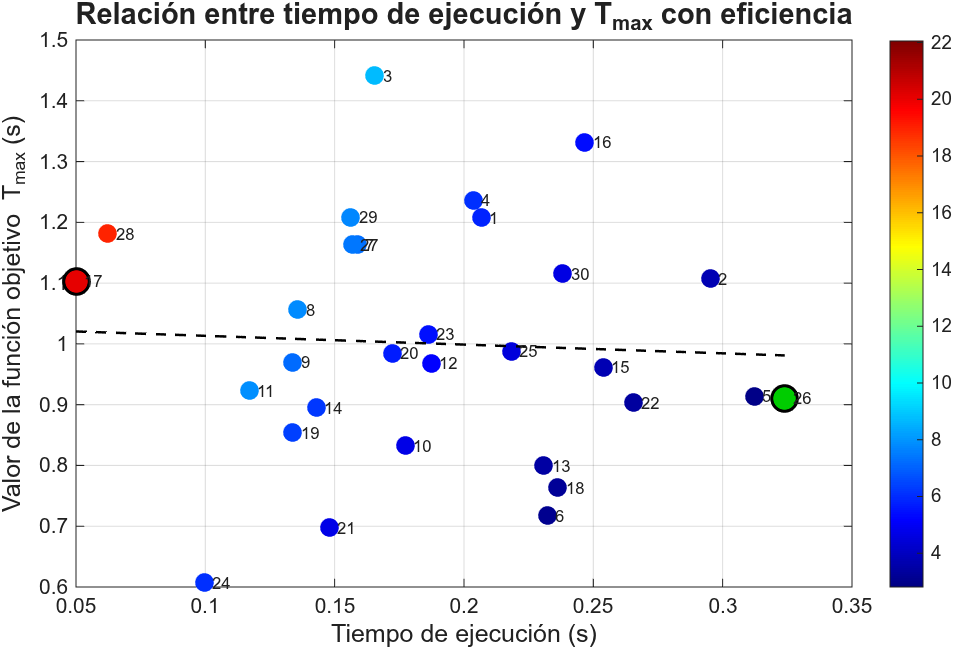
\includegraphics[scale=0.6]{Images/tema2/scatter_plot_propuesta.png}
  \caption{Diagrama de dispersión propuesto para la evaluación de la eficiencia de las soluciones. 
  Cada círculo representa una solución cuyo número adjunto corresponde con el número de ejecución, 
  el color de las soluciones se refiere a la eficiencia de las mismas, los círculos con borde negro
  representan las peor y mejor solución, en color rojo y verde, respectivamente, y la recta punteada 
  la línea de tendencia.}
  \label{fig:scatterPlotPropuesta}
\end{figure}

\subsection*{Conclusiones (expectativas)}
\addcontentsline{toc}{subsection}{Conclusiones (expectativas)}
Se espera que el Temple Simulado sea capaz de identificar configuraciones de
\textit{rendezvous} que reduzcan el valor de $T_{\max}$ y, por tanto, mejoren la
sincronización entre los dos robots. Dado que el problema combina posiciones,
orientaciones y factores de velocidad, el algoritmo debería explorar de forma
eficiente regiones del espacio de búsqueda que no serían accesibles mediante
métodos deterministas o gradientes locales. \\

Además, se busca ajustar automáticamente los factores de velocidad para compensar las
diferencias cinemáticas entre robots y el eje lineal. \\

Se considerará que el Temple Simulado constituye una estrategia válida para la
optimización del \textit{rendezvous} cooperativo si logra reducir $T_{\max}$ de
forma estable y reproducible respecto del punto de partida, si muestra 
estabilidad de los valores finales en las últimas iteraciones, es decir, convergencia,
y si el diagrama de dispersión muestra una tendencia alineada con el objetivo del problema.
\newpage
\datos{color}{}{}
\section*{Revisión y desarrollo de la propuesta técnica de búsqueda local}
\addcontentsline{toc}{section}{Revisión y desarrollo de la propuesta técnica de búsqueda local y propuesta final}
En esta sección se describen las correcciones introducidas a partir de la revisión del profesorado
sobre la propuesta inicial de búsqueda local. Tras incorporar dichas modificaciones se observó que
el algoritmo de optimización comenzaba a mostrar un nivel significativo de ruido en la evaluación del coste.
Este ruido estaba asociado a la elevada dimensionalidad del espacio de búsqueda que introducía
soluciones no factibles desde el inicio. \\

Para mitigar este efecto, se ha realizado un análisis específico orientado a reducir la dimensionalidad 
efectiva del problema y filtrar las soluciones no válidas antes de la optimización. En concreto, se 
ha resuelto el problema diseñando una arquitectura de dos niveles.

\subsection*{Revisión del profesorado}
\addcontentsline{toc}{subsection}{Revisión del profesorado}
En la revisión de la propuesta inicial, el profesorado señaló dos aspectos
que debían corregirse en el diseño del Temple Simulado. En primer lugar, se indicó
que la temperatura inicial \(T_0\) no debía fijarse de forma arbitraria, sino
sintonizarse en función de la escala real de los incrementos de coste
\(\Delta J\) observados en las primeras iteraciones. El objetivo es garantizar
una tasa de aceptación inicial elevada (del orden del 80--90\%) para
empeoramientos, evitando que el algoritmo se comporte como una búsqueda ávida
(Hill Climbing) si \(T_0\) resulta demasiado baja para la magnitud de la función
de mérito. \\

En segundo lugar, se advirtió que el uso de una única desviación típica
\(\sigma = 0.1\) para todas las variables no era adecuado, ya que posiciones,
orientaciones y factores de velocidad operan en escalas muy distintas. Esto puede
provocar mutaciones desbalanceadas: algunas variables se hiper-mutaban mientras
otras permanecían prácticamente estáticas. Por ello, se recomendó definir
desviaciones típicas diferenciadas (\(\sigma_p, \sigma_q, \sigma_s\)) adaptadas
a la naturaleza y rango de cada tipo de variable. \\

Estas observaciones se han incorporado en la actualización de la propuesta
mediante un rediseño en dos niveles. En el Nivel 1 se filtran puntos
cinemáticamente válidos (IK + manipulabilidad), reduciendo la dimensionalidad
efectiva del problema y eliminando gran parte del ruido en la evaluación. En el
Nivel 2 se emplea un Temple Simulado con parámetros \(\sigma\) diferenciados y
una temperatura inicial \(T_0\) ajustada a la magnitud real de \(\Delta J\),
logrando así un comportamiento más estable, eficiente y coherente con la teoría
del método.

\subsection*{Diseño de la búsqueda de la solución}
\addcontentsline{toc}{subsection}{Diseño de la búsqueda de la solución}
Con la propuesta inicial se podían generar vecinos que estuvieran fuera del espacio de trabajo 
de los robots, por lo que desde el inicio eran puntos no factibles. Su perturbación para la generación 
de nuevos vecinos no incluía ningún mecanismo que pudiera acerca el nuevo punto al espacio de trabajo. 
Por tanto, el algoritmo tenía una alta probabilidad de ser incapaz de explorar correctamente soluciones 
factibles. \\

Además, la naturaleza del problema implica que un mismo punto en el espacio tenga comportamientos diferentes 
según los perfiles de velocidad y la posición del raíl aplicada. Consecuentemente, los perfiles de
velocidad y la posición del raíl tienen que ser optimizados para cada punto factible, y después, optimizar 
esas soluciones completas, es decir, quedarse con la mejor. \\

Dado este análisis, se ha propuesto una arquitectura basada en dos niveles. En el primer nivel se generan 
los vecinos y la información que será introducida al algoritmo de Temple Simulado. Estos vecinos se generan
dentro de la intersección del espacio de trabajo de ambos robots para cuando el raíl está no se ha desplazado,
puesto que en esta posición la intersección es máxima. Asimismo, estos puntos son cinemáticamente factibles,
se han fijado las orientaciones acorde a la \autoref{fig:conf} y se obtiene el rango de posiciones del ŕail
para el que el robot B puede alcanzar la posición generada. \\

En el segundo nivel, el algoritmo de Temple Simulado optimiza los perfiles de velocidad y la posición del raíl
para la posición factible generada, generando vecinos en las variables a optimizar. En el caso del raíl,
su generación de vecinos está acotada al rango obtenido en el nivel anterior, puesto que garantiza que sea alcanzable.\\

Tras resolver exitosamente el problema con este enfoque, se ha observado lo posibilidad de aplicar otra 
metodología:
establecer un mecanismo de evaluación que determine cómo de lejos se encuentra un punto en el espacio del 
espacio de trabajo factible para que el algoritmo de Temple Simulado sea capaz de converger hacia puntos factibles.
No obstante, como ya se había resuelto el problema y dado que se trata de un proyecto académico de una asignatura
de 6 créditos ECTS, este nuevo enfoque se plantea como línea futura. \\


\subsection*{Diseño del algoritmo}
\addcontentsline{toc}{subsection}{Diseño del algoritmo}

\subsubsection*{Representación de las soluciones}
Cada solución candidata se representa como un vector continuo:
\[
\mathbf{x} =
(\mathbf{p}_A,\mathbf{p}_B,
\mathbf{q}_A,\mathbf{q}_B,
s_A,s_B,s_{rail})
\in \mathbb{R}^{18},
\]

donde $\mathbf{p}_A \in \mathbb{R}^3, \mathbf{p}_B \in \mathbb{R}^4$ son las posiciones objetivo de cada robot en el marco
del mundo, incluyendo la posición del raíl optmizada para el robot B,
$\mathbf{q}_A, \mathbf{q}_B \in S^3$ son cuaterniones unitarios que representan orientaciones de cada efector y
$s_A, s_B, s_{rail} \in (0,1]$ son los factores de velocidad de cada robot y del motor lineal de desplazamiento. \\

Con el objetivo de simplificar el problema, el marco del mundo coincide con el marco del robot A, la base
del robot B se encuentra desplaza ($0.75 + \textit{posición del raíl}$) metros en el eje $X$ (cumpliendo con 
la \autoref{fig:conf}, donde el raíl puede tomar cualquier valor entre $[0.0, 0.70]$), y las orientaciones
son fijas en $\mathbf{q}_A = (0.70710678, 0.70710678, 0.0, 0.0)$ y $\mathbf{q}_B = (0.0, -0.38268343, 0.0, 0.92387953)$. \\

Para facilitar la interpretación de dichas orientaciones, se presentan a continuación sus valores en \textit{RPY}
(\textit{Roll}, \textit{Pitch}, \textit{Yaw}). En el caso del robot A ($\mathbf{q}_A$),
la orientación deseada corresponde a los ángulos en radianes \((\pi,\ \pi/2,\ 0)\), lo que
equivale a una rotación de \(180^\circ\) alrededor del eje \(x\) seguida de una
rotación de \(90^\circ\) alrededor del eje \(y\). Para el robot B ($\mathbf{q}_B$), la
orientación especificada es \((0,\ -\pi/2,\ 0)\), es decir, una rotación de
\(-90^\circ\) alrededor del eje \(y\).


\subsubsection*{Operadores de vecindad}
En primer lugar, se presenta la generación de vecinos para el nivel 1 de la arquitectura planteada.
En este nivel el operador de vecindad ya no se basa en perturbaciones gaussianas. En su lugar, se ha
diseñado un generador de vecinos específico para la naturaleza geométrica y cinemática del problema, 
cuyo objetivo es producir únicamente puntos factibles para ambos robots antes de iniciar la optimización
temporal del nivel 2. \\

El proceso consta de tres etapas principales:

\begin{enumerate}
    \item \textbf{Muestreo geométrico en el espacio de trabajo.}
    Se genera un punto candidato \(p_A\) mediante muestreo uniforme dentro de la
    intersección de los cilindros de alcance de los dos robots. A partir de él
    se define automáticamente el punto correspondiente del robot~B como
    \(p_B = p_A + \textit{offset}\), garantizando la distancia relativa requerida
    entre ambos efectores, es decir, cumpliendo las restricciones definidas sobre la separación
    final en el mundo y la posición de enfrentamiento. \\

    Los cilindros de alcance de los dos robots viene dado por el fabricante: un radio de 
    $0.762$ metros y una altura de $1.029$ metros. \\

    En la \autoref{fig:muestreo} se observa visualmente la generación de estos puntos 
    factibles.

    \begin{figure}[H]
        \centering
        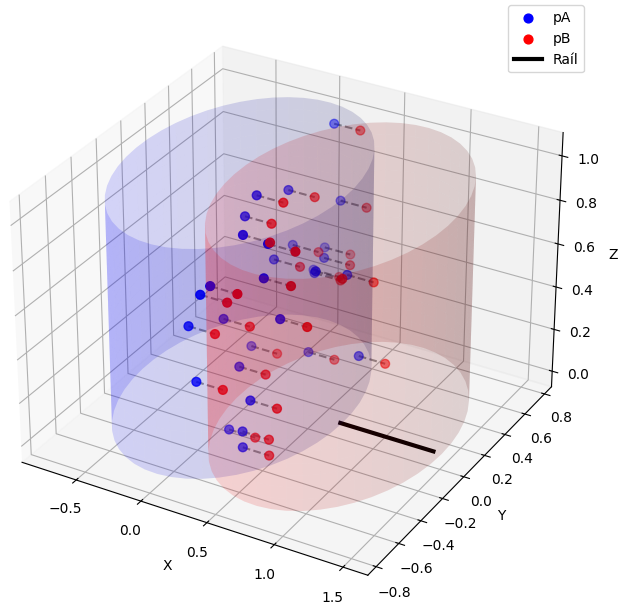
\includegraphics[scale=0.4]{Images/muestreo.png}
        \caption{Visualización 3D de la generación de puntos espaciales factibles.}
        \label{fig:muestreo}
    \end{figure}

    \item \textbf{Comprobación de factibilidad del raíl.}
    Para el punto \(p_B\) se calcula el intervalo de posiciones del raíl
    \([r_{\min}, r_{\max}]\) que permiten alcanzarlo. Si dicho intervalo es
    vacío, el punto se descarta. En caso contrario, se selecciona un valor
    intermedio \(p_{\text{Rail}}\) para evaluar la cinemática inversa.

    \item \textbf{Filtrado cinemático (IK + manipulabilidad).}
    Se resuelven las cinemáticas inversas de ambos robots para las orientaciones
    deseadas y se comprueba que las soluciones articulares obtenidas presentan
    una manipulabilidad superior a un umbral mínimo. Solo si se cumplen ambas
    condiciones, el punto se acepta como vecino válido. Este filtrado corresponde 
    con la restricción de singularidades.

    Del trabajo realizado en la asignatura de Robótica Industrial del Máster 
    se conoce que los valores típicos de manipulabilidad en el espacio de trabajo
    de ambos robots presentan valores superiores a \(0.05\), mientras que las 
    configuraciones cercanas a singularidades caen por debajo de dicho rango. 
    Por este motivo se ha fijado un umbral conservador en $0.08$.
\end{enumerate}

En segundo lugar, el operador de vecindad del nivel 2 sí se basa en perturbaciones 
gaussianas, pero aplicadas únicamente a las variables temporales. Estas variables operan
en rangos similares, por lo que ambas perturbaciones sí pueden utilizar la misma 
desviación típica, $\sigma = 0.05$, que permite explorar
variaciones apreciables en el tiempo de ejecución sin producir saltos
excesivos que desestabilicen el Temple Simulado.

\begin{itemize}
    \item \textbf{Factores de velocidad}.  
    Cada velocidad escalar se perturba mediante
\[
        s_r' = s_r + \mathcal{N}(0,\sigma_s^2),
        \qquad r \in \{A, B, \text{Rail}\},
    \]
    seguida de un truncamiento para garantizar la factibilidad física:
\[
        s_r' \leftarrow \min\big(1,\max(0,s_r')\big).
    \]

    \item \textbf{Posición del raíl}.  
    La posición final del raíl se perturba mediante
\[
        p_{\text{Rail}}' = p_{\text{Rail}} + \mathcal{N}(0,\sigma_{\text{rail}}^2),
    \]
    y posteriormente se proyecta al intervalo factible calculado en el nivel 1:
\[
        p_{\text{Rail}}' \leftarrow
        \min\big(r_{\max},\max(r_{\min},p_{\text{Rail}}')\big).
    \]
    Esta operación garantiza que el robot~B pueda alcanzar el punto \(p_B\) tras
    la mutación.

\end{itemize}

\subsubsection*{Gestión de restricciones}
Como se ha venido explicando, la arquitectura implementada junto con los operadores 
de vecindad cumplen la mayoría de las restricciones gracias a la incorporación 
del conocimiento del dominio. De esta manera, la única restricción a verificar por 
el algoritmo del Temple simulador será la sincronización temporal:

\[\big|t_A(\mathbf{p}_A,\mathbf{q}_A,\mathbf{s}_A)-t_B(\mathbf{p}_B,\mathbf{q}_B,\mathbf{s}_B,\mathbf{s}_{rail})\big| \le \Delta t_{\max}\].

Por tanto, la evaluación de cada solución se basa en esta diferencia temporal:
cuanto más próximos estén ambos tiempos, mejor será la calidad de la solución. Se ha 
modificado la función de penalización correspondiente para cumplir con 
este planteamiento:
\[
P_{\text{sync}}(\Delta t) =
\begin{cases}
\left(\dfrac{\Delta t}{\Delta t_{\max}}\right)^2,
& \text{si } \Delta t \le \Delta t_{\max}, \\
1 + \left(\dfrac{\Delta t - \Delta t_{\max}}{\Delta t_{\max}}\right)^2,
& \text{si } \Delta t > \Delta t_{\max}.
\end{cases}
\]

Es importante destacar que con esta modificación la restricción de sincronización
no se aplica como un filtro duro que descarte soluciones que excedan el umbral
\(\Delta t_{\max}\). En su lugar, la restricción se incorpora mediante una
\emph{penalización continua} que permite al Temple Simulado seguir explorando el
espacio de soluciones incluso cuando la diferencia temporal es superior al
límite deseado. De este modo se evita la aparición de zonas ciegas en la función
de mérito y se mantiene un gradiente útil para guiar la búsqueda. \\

De este modo, el Temple Simulado explora libremente el espacio de búsqueda,
mientras que la función de evaluación guía la convergencia hacia soluciones que
cumplen las restricciones, en este caso, la sincronización temporal.

\subsection*{Configuración de parámetros}
\addcontentsline{toc}{subsection}{Configuración de parámetros}

Conociendo el modelo del tiempo de ejecución de cada robot utilizado, descrito
en la propuesta de esta memoria, los datos geométricos del problema, el
alcance máximo de los robots y el recorrido máximo del raíl, es posible acotar
de forma aproximada los tiempos de ejecución:


\[
t_r \in [t_{\min}, t_{\max}] \approx [0.5\,\text{s},\, 2.5\,\text{s}].
\]



En consecuencia, la desincronización máxima teórica entre ambos robots se sitúa
en el orden de


\[
\Delta t_{\max}^{\text{teo}} \approx t_{\max} - t_{\min} \approx 2\,\text{s}.
\]



Sin embargo, el operador de vecindad del nivel 2 no genera saltos extremos, sino
pequeñas variaciones en los factores de velocidad y en la posición del raíl
(\(\sigma_s = 0.05\), \(\sigma_{\text{rail}} = 0.05\)). Esto implica que la
diferencia de tiempos entre soluciones vecinas se sitúa típicamente en el orden
de unas pocas décimas de segundo, lo que se traduce en una variación de coste
esperada:


\[
\Delta J_{\text{esp}} \sim P_{\text{sync}}(\Delta t) - P_{\text{sync}}(\Delta t')
\qquad\Rightarrow\qquad
\Delta J_{\text{esp}} \in [0.1,\, 0.3].
\]



Esta estimación permite sintonizar la temperatura inicial del Temple Simulado
sin necesidad de recurrir a ejecuciones preliminares ni a ajustes empíricos. El
objetivo de la temperatura inicial es garantizar una probabilidad de aceptación
elevada (80--90\%) para empeoramientos típicos de magnitud
\(\Delta J_{\text{esp}}\). Utilizando la relación clásica del Temple Simulado,


\[
T_0 = -\frac{\Delta J_{\text{esp}}}{\ln(p_0)}, \qquad p_0 \in [0.8,0.9],
\]


y tomando como referencia un valor medio \(\Delta J_{\text{esp}} \approx 0.2\),
se obtiene:


\[
T_0 \approx -\frac{0.2}{\ln(0.85)} \approx 0.96.
\]



Por simplicidad se adopta finalmente
\[
T_0 = 1,
\]

valor coherente con la escala temporal del problema y que evita que el algoritmo
degenere en una búsqueda puramente ávida en las primeras iteraciones. \\

Por otra parte, el enfriamiento empleado es de tipo geométrico, 
\(T_{k+1} = \alpha\, T_k\), por ser el más habitual en problemas continuos y por su buena 
relación entre simplicidad y estabilidad. La elección del factor de enfriamiento \(\alpha\) 
se ha realizado en función del número total de iteraciones disponibles y de la escala de la función
de mérito. \\

Se define un máximo de \texttt{max\_iters} \(= 300\)
iteraciones, por lo que el factor de enfriamiento debe garantizar que la temperatura se
mantenga suficientemente alta durante las primeras fases (para permitir
exploración) y que descienda de forma progresiva hacia valores cercanos a cero
en las últimas iteraciones (para favorecer la explotación). Para un enfriamiento
geométrico, la temperatura tras \(N\) iteraciones es:
\[
T_N = T_0\, \alpha^N.
\]

Imponiendo que la temperatura final sea aproximadamente dos órdenes de magnitud
menor que la inicial, es decir, \(T_N \approx 10^{-2} T_0\), se obtiene:
\[
\alpha^N \approx 10^{-2}
\quad\Rightarrow\quad
\alpha \approx 10^{-2/N}.
\]

Sustituyendo \(N = 300\) se obtiene:
\[
\alpha \approx 10^{-2/300} \approx 0.95.
\]

Por tanto, el valor \(\alpha = 0.95\) no es arbitrario, sino que garantiza un
descenso suave de la temperatura a lo largo de las 300 iteraciones disponibles,
manteniendo capacidad exploratoria en las primeras fases y favoreciendo la
convergencia en las finales.\\

El proceso de optimización temporal utiliza un máximo de
\texttt{max\_iters} \(= 300\) iteraciones. Este valor sustituye al esquema
clásico de dos bucles del Temple Simulado (con \(K\) temperaturas y \(L\)
vecinos por temperatura), debido a la propia naturaleza de la arquitectura en
dos niveles. \\

En un Temple Simulado convencional, el esquema \(K \times L\) es necesario para
compensar la presencia de un espacio de búsqueda ruidoso, con restricciones
complejas y con una elevada probabilidad de generar soluciones no factibles.
Sin embargo, en la arquitectura propuesta, el nivel 1 garantiza que todas las
soluciones que llegan al nivel 2 son geométrica y cinemáticamente factibles,
están libres de singularidades y cumplen las restricciones del raíl. Como
consecuencia, el espacio de búsqueda del nivel 2 es continuo, de baja
dimensionalidad y completamente factible, por lo que no requiere un proceso de
exploración tan intensivo. \\

Además, el operador de vecindad del nivel 2 produce variaciones pequeñas y
controladas en los parámetros temporales, lo que reduce drásticamente el ruido
en la función de mérito. En este contexto, el uso de un único bucle con un
número total de iteraciones fijo resulta más eficiente y permite un control más
directo sobre el coste computacional. \\

En la práctica, 300 iteraciones proporcionan un equilibrio adecuado entre
exploración y explotación, permitiendo alcanzar convergencia estable sin
incrementar de forma excesiva el tiempo de cómputo. En otras palabras, 
se probarán 300 combinaciones de soluciones por cada punto del nivel 1, siendo un 
número adecuado dado el amplio espacio de búsqueda combinatorio definido 
por las cuatro variables continuas a optimizar en el Temple Simulado.

\begin{comment}
    \begin{itemize}
    \item Temperatura inicial: $T_0 = 1$
    \item Factor de enfriamiento: $\alpha = 0.95$
    \item Iteraciones (movimientos) por temperatura: $L = 50$
    \item Número máximo de iteraciones (temperaturas): $K = 200$
    \item Desviación del operador de vecindad: $\sigma = 0.1$
\end{itemize}
\end{comment}

\subsection*{Diseño experimental}
\addcontentsline{toc}{subsection}{Diseño experimental}
El plan de experimentación constará de la optimización de 
30 puntos espaciales diferentes. \\

Las soluciones se evaluarán mediante tres métricas: calidad, tiempo de ejecución y número de evaluaciones.
La calidad registra el mejor y peor 
valor final de $T_{\max}$, la media, la desviación típica y el intervalo de confianza. El tiempo
de ejecución mide el tiempo total de \textit{CPU} y se considera con la calidad de la
solución lograda. Esta consideración se realizará a través de un diagrama de dispersión, como 
el de la Figura \ref{fig:scatterPlotPropuesta}, y 
un valor de eficiencia calculado: $E = \frac{T_{max}}{\text{tiempo}}$. Por último,
el número de evaluaciones anota la iteración en la que se alcanzó el mejor valor. \\

\subsection*{Resultados}
\addcontentsline{toc}{subsection}{Resultados}
Se han realizado modificaciones sobre la representación de resultados propuesta para evitar 
la redundancia de información. La \autoref{tab:tema2_tabla1} y la \autoref{fig:scatterPlotPropuesta}
contenían información duplicada y además, la tabla resultaría difícil de leer por su gran volumen 
de datos. Por ello, se ha decidido suprimir la tabla. \\

Además, con el objetivo de analizar la estabilidad del método, evaluar la variabilidad entre
ejecuciones y estudiar el comportamiento dinámico del algoritmo durante el proceso de optimización
se añaden dos diagramas de cajas y la curva media de convergencia. Un diagrama de caja representa
el valor de $T_{\text{máx}}$ y otro los diferentes 
valores de la coordenada $x$ de los puntos A y B, puesto que las coordenadas $y$ y $z$ están fijadas
durante el proceso de optimización. \\

Por otro lado, con los cambios realizados ya no existen soluciones infactibles, por lo que no es necesario
registrar el porcentaje de soluciones factibles obtenidas por el algoritmo.\\

El mejor resultado obtenido viene definido por $T_{\max} = 0.96\, s$ con 
el vector número 7 (recordar que las orientaciones están previamente fijadas): 
\[(\mathbf{p}_A,\mathbf{p}_B,
\mathbf{q}_A,\mathbf{q}_B,
s_A,s_B,s_{rail}) = 
((0.35, 0.12, 0.15), (0.55, 0.12, 0.15, p_{\text{raíl}} = 0.5), qA, qB, 0.41, 1, 0.84)\]

Los resultados de la \autoref{tab:tema2_tabla2} muestran que el algoritmo presenta un comportamiento
estable y consistente a lo largo de las 30 ejecuciones realizadas. El valor medio de $T_{\max}$ es
de 1.67\,s, con una desviación típica moderada (0.50\,s), lo que indica que la variabilidad entre
ejecuciones es relativamente baja. El mejor caso alcanza un tiempo de 0.96\,s, mientras que el peor
se sitúa en 2.88\,s, lo que define el rango completo de rendimiento del método. El intervalo de 
confianza al 95\,\% $[1.49,\,1.88]$\,s confirma que, con alta probabilidad, el algoritmo converge
de forma consistente en torno a valores próximos a la media. \\

Por otro lado, el tiempo medio de ejecución del proceso completo es de 0.83\,s, lo que demuestra
que el método es computacionalmente eficiente y adecuado para escenarios donde se requiere 
optimización rápida. \\

De forma complementaria, el diagrama de cajas de la \autoref{fig:cajaT} 
muestra que la mayor parte de las soluciones de $T_{\max}$ se concentran en un intervalo 
relativamente estrecho. El rango intercuartílico se sitúa aproximadamente entre 1.25\,s y 1.90\,s, 
lo que indica que el 50\% central de las ejecuciones produce soluciones de calidad similar.
El bigote inferior desciende hasta aproximadamente 1.00\,s, mientras que el superior alcanza
valores cercanos a 2.90\,s, lo que refleja la presencia de ejecuciones más extremas, tanto muy
buenas como menos favorables. No obstante, la ausencia de valores atípicos sugiere que
estas variaciones se encuentran dentro del comportamiento esperado del método.

%En conjunto, el diagrama evidencia que el algoritmo es estable, con una dispersión moderada y sin
%comportamientos anómalos.

\begin{table}[H]
\centering
\begin{tabular}{|l|c|}
\hline
\textbf{Métrica} & \textbf{Valor} \\
\hline
Media de $T_{\max}$ & 1.67 s \\
Desviación típica & 0.5 \\
Mejor valor (mínimo) & 0.96 s \\
Peor valor (máximo) & 2.88 s \\
Intervalo de confianza 95\% & [1.49, 1.88] s\\
Tiempo medio de ejecución (s) & 0.83 s \\
\hline
\end{tabular}
\caption{Métricas agregadas calculadas sobre las 30 ejecuciones.}\label{tab:tema2_tabla2}
\end{table}

\begin{figure}[H]
  \centering
  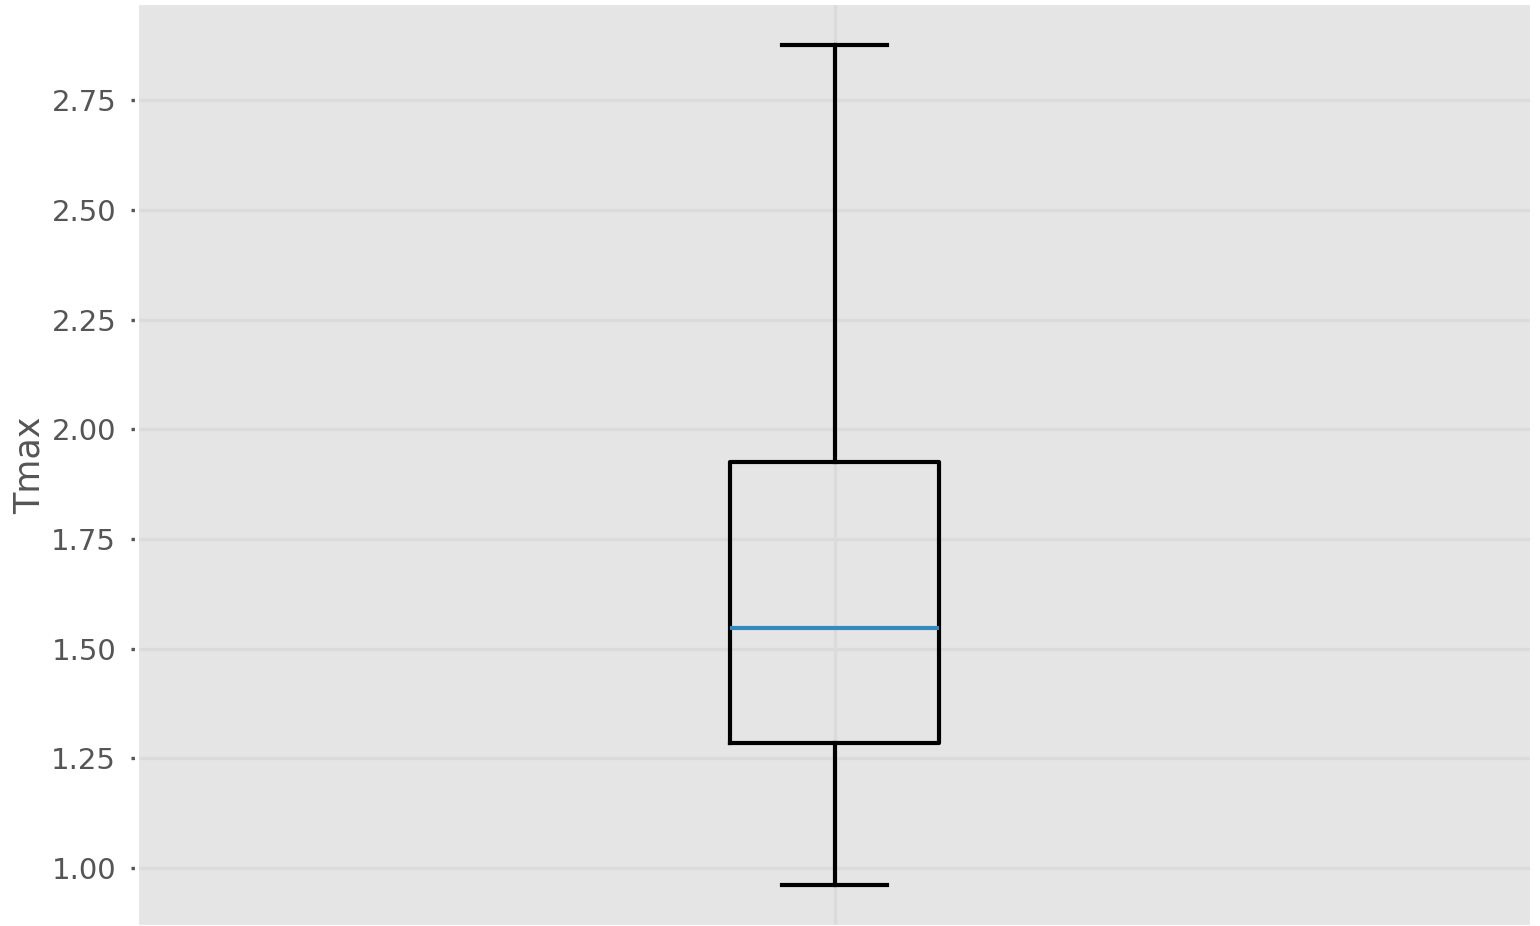
\includegraphics[scale=0.17]{Images/tema2/boxplot_Tmax.png}
  \caption{Diagrama de caja de la solución temporal.}
  \label{fig:cajaT}
\end{figure}

También resulta interesante evaluar la variabilidad en los puntos espaciales explorados. En 
la \autoref{fig:cajaP} se presenta el diagrama de caja para la coordenada $x$ de los puntos A 
y B. La mayoría de las soluciones se agrupan en el intervalo $[0.2, 0.4]$ metros y $[0.4, 0.6]$
metros, lo que
induce a pensar que esas zonas son las regiones más estables, alcanzables o cinemáticamente factibles
para los robots. En la \autoref{fig:visP} se visualizan en tres dimensiones los 30 puntos explorados.

\begin{figure}[H]
  \centering
  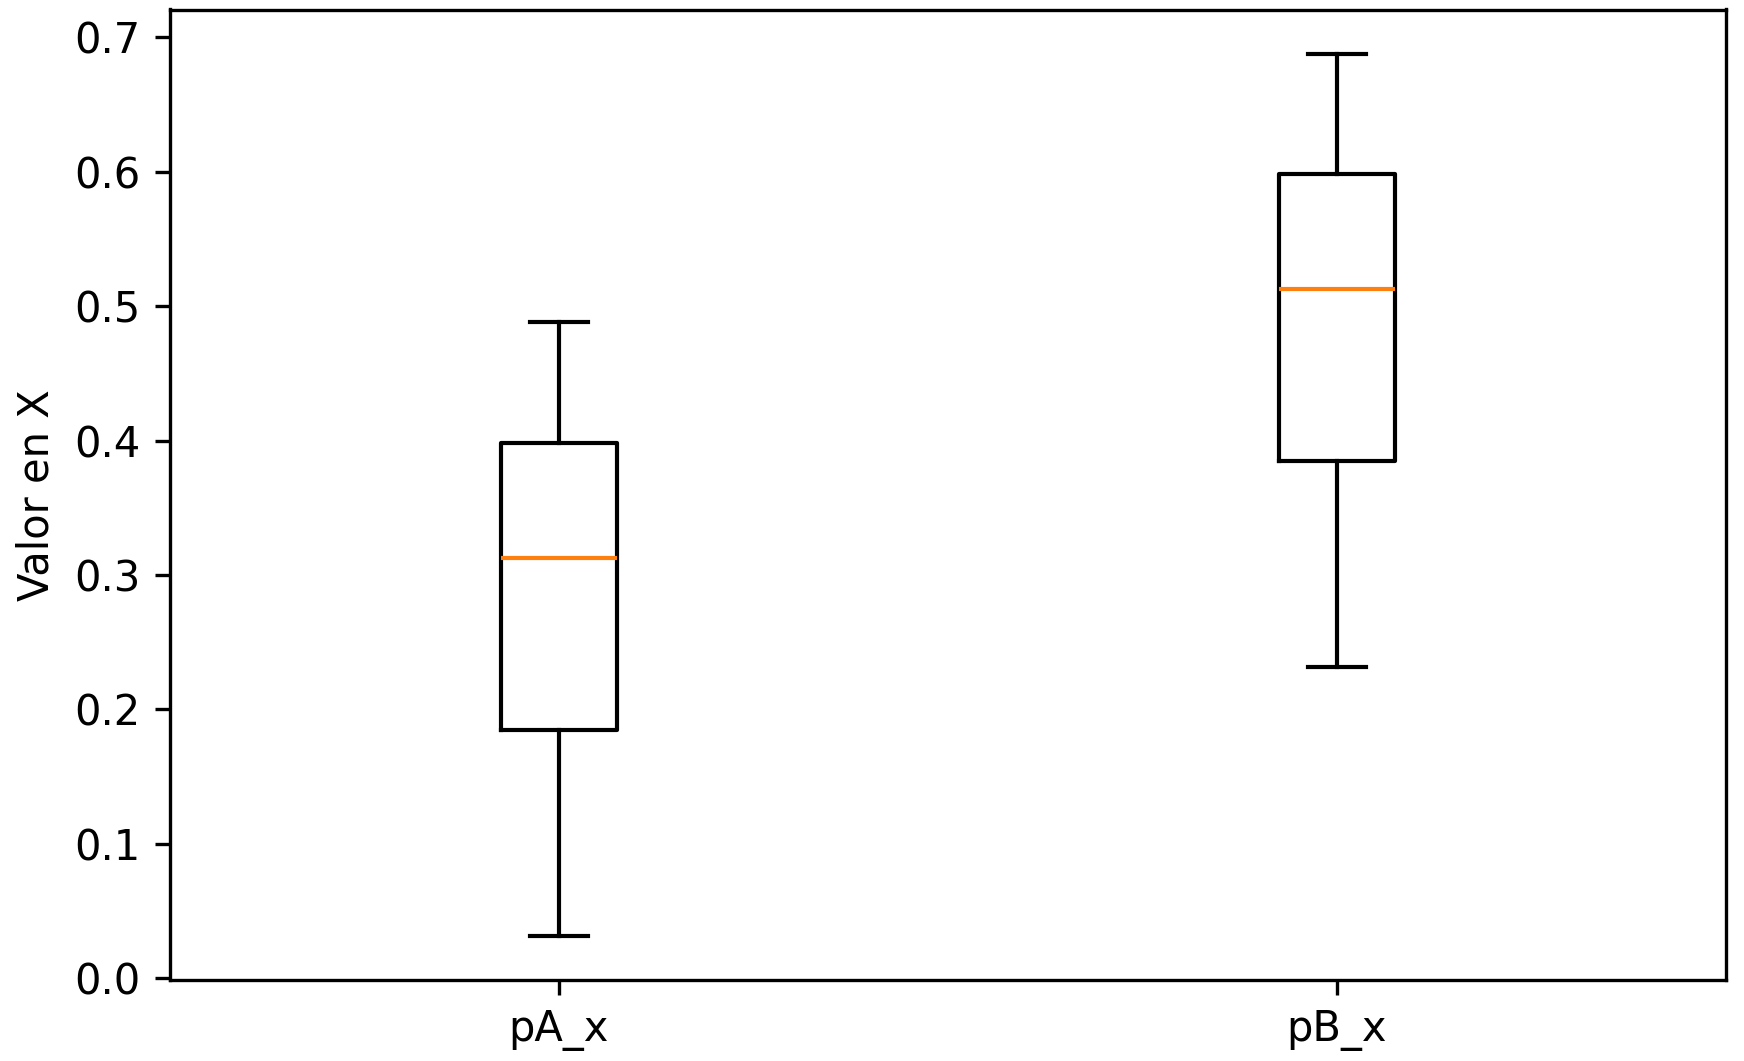
\includegraphics[scale=0.14]{Images/tema2/boxplot_pA_x_pB_x.png}
  \caption{Diagrama de caja del punto espacial.}
  \label{fig:cajaP}
\end{figure}
\begin{figure}[H]
  \centering
  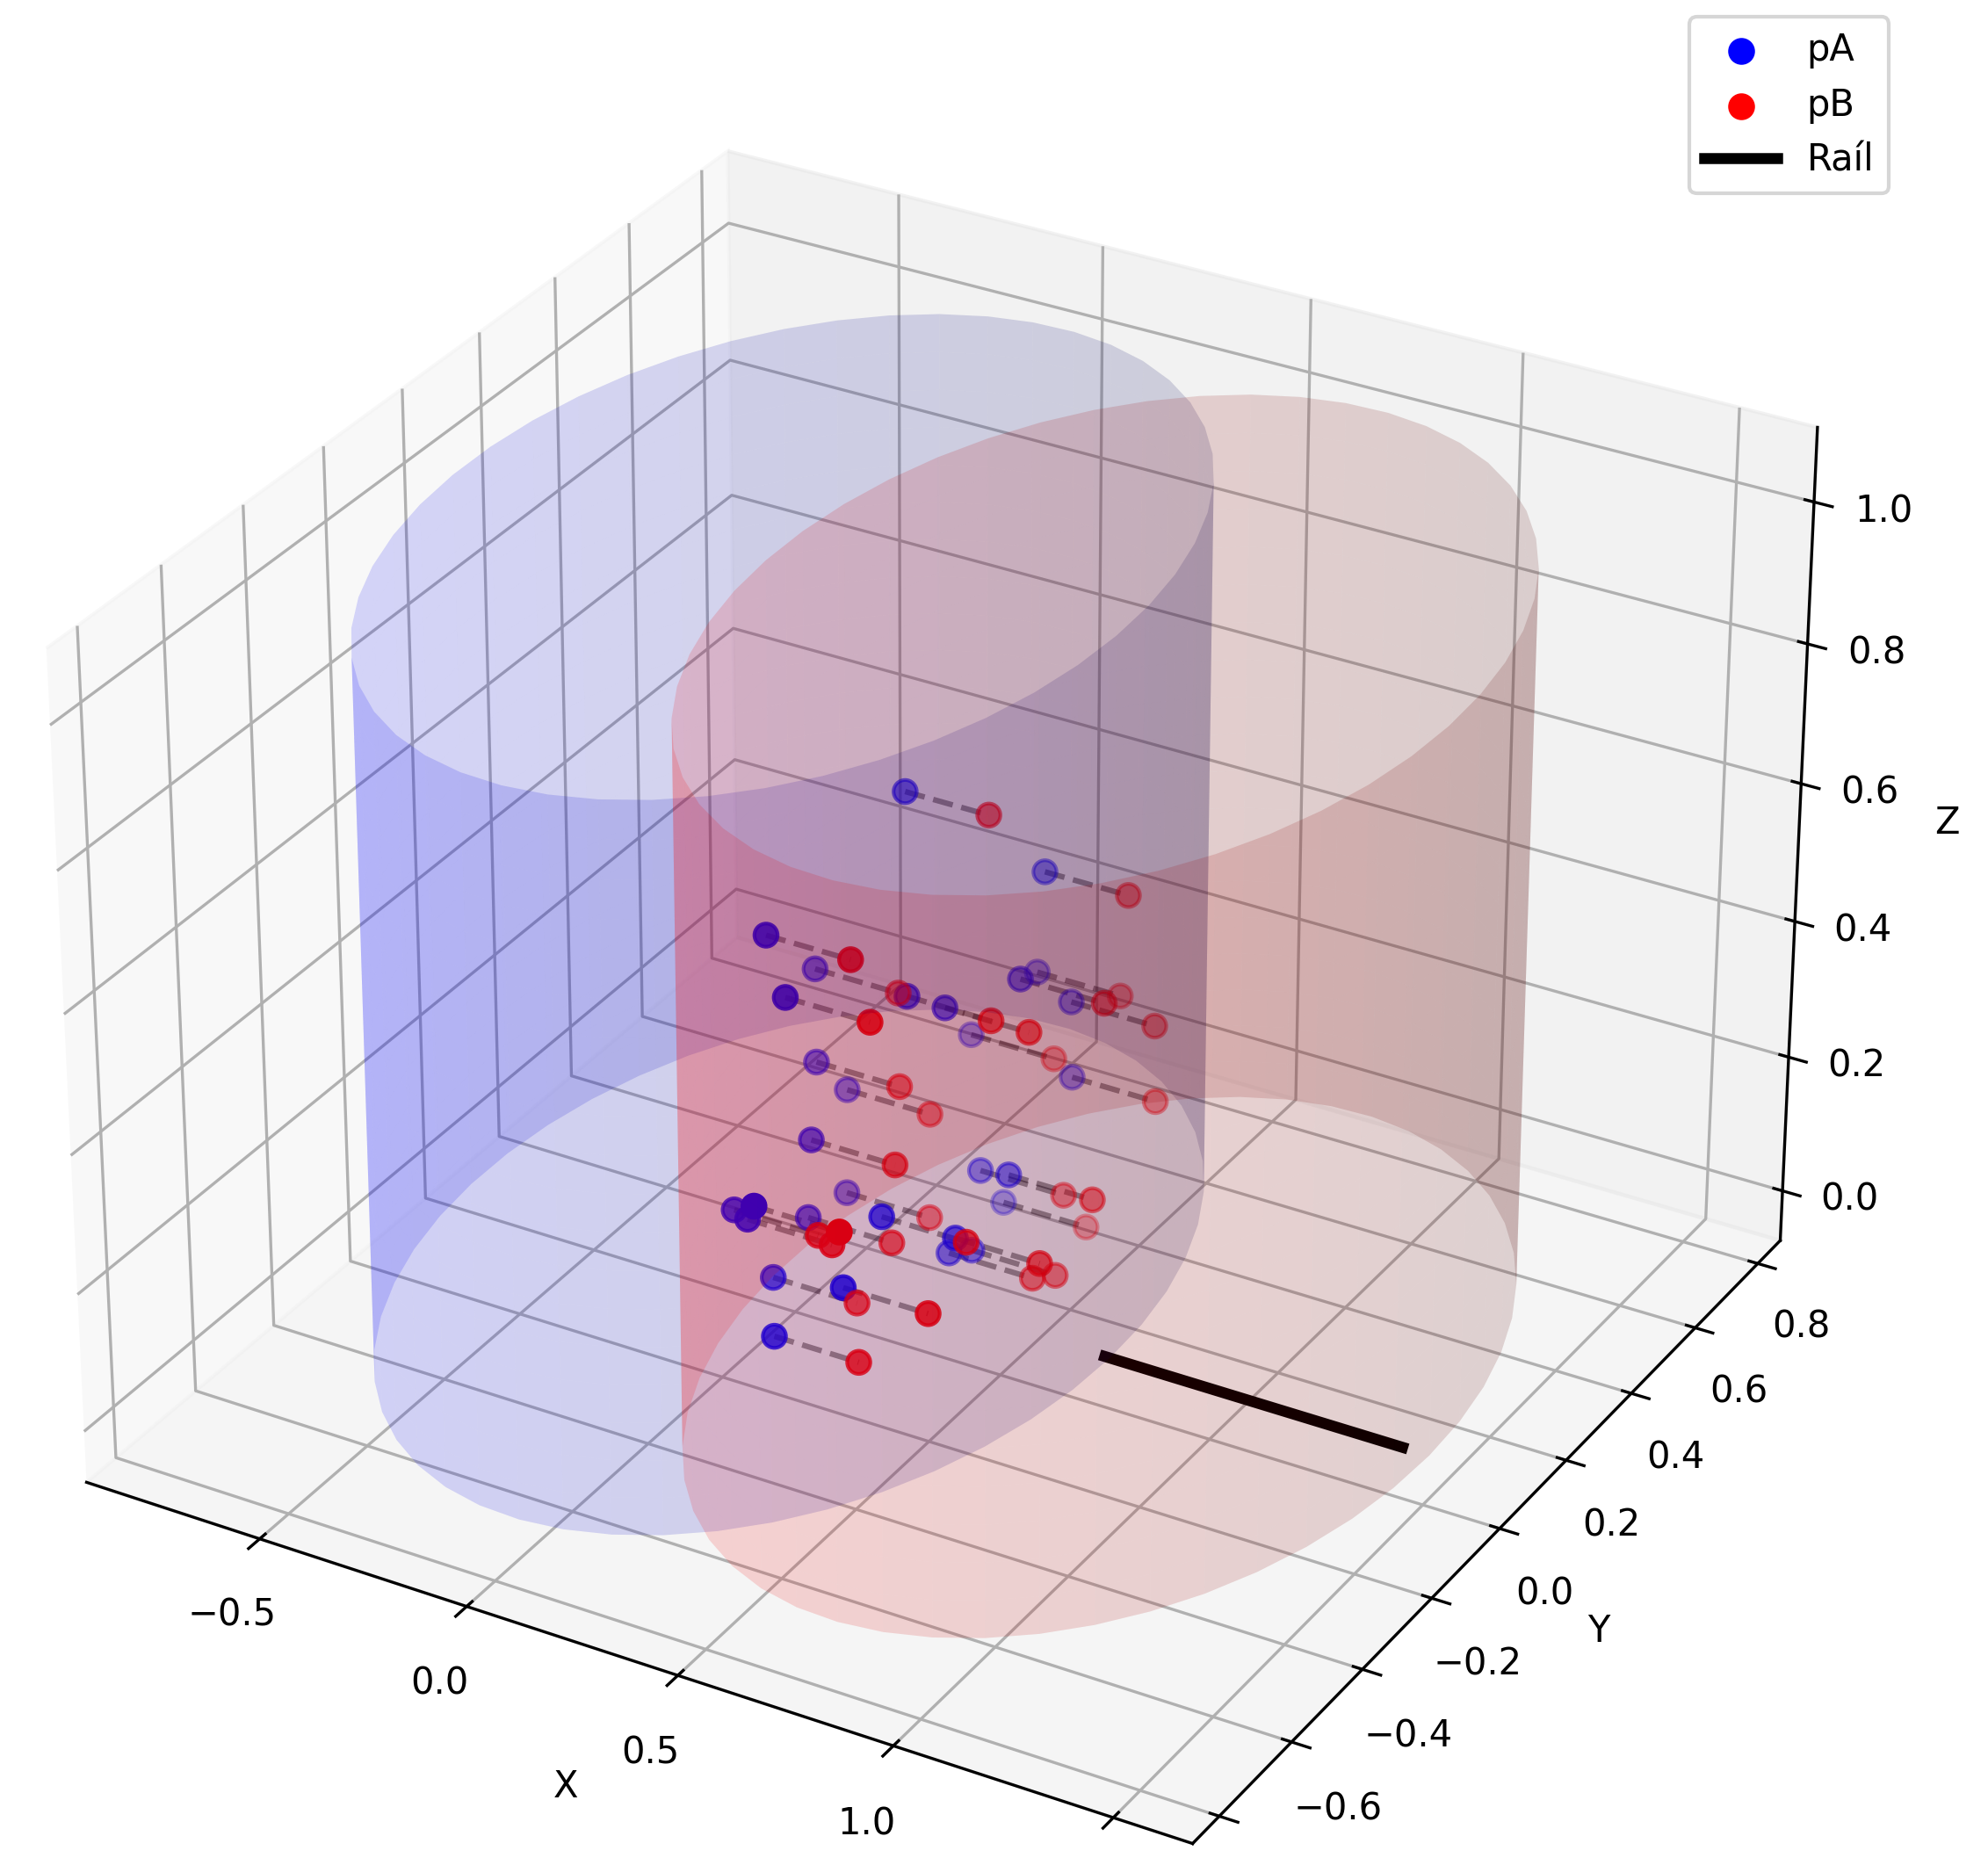
\includegraphics[scale=0.1]{Images/tema2/visualizacion_pA_pB.png}
  \caption{Visualización de los puntos espaciales factibles optimizados.}
  \label{fig:visP}
\end{figure}

En lo relativo a la eficiencia, la \autoref{fig:scatterPlot} muestra que la métrica propuesta no
aporta nada útil a la evaluación, ya que las soluciones con mayor tiempo de desplazamiento de 
los robots calculada en el menor tiempo de computación tiene una mayor eficiencia. Esta relación
no aporta ningún significado. La única información de interés que se obtiene es que el tiempo máximo
de ejecución es de 3 segundos por punto espacial. Consecuentemente, resulta necesario definir otra métrica. En este 
caso, se ha optado por la curva de convergencia del método. \\

Esta curva se presenta en la \autoref{fig:curvaMedia}, donde se observa que el algoritmo ha  
convergido a las 80 iteraciones de las 300 que se realizan, ya que la penalización es prácticamente 
nula.
\begin{figure}[H]
  \centering
  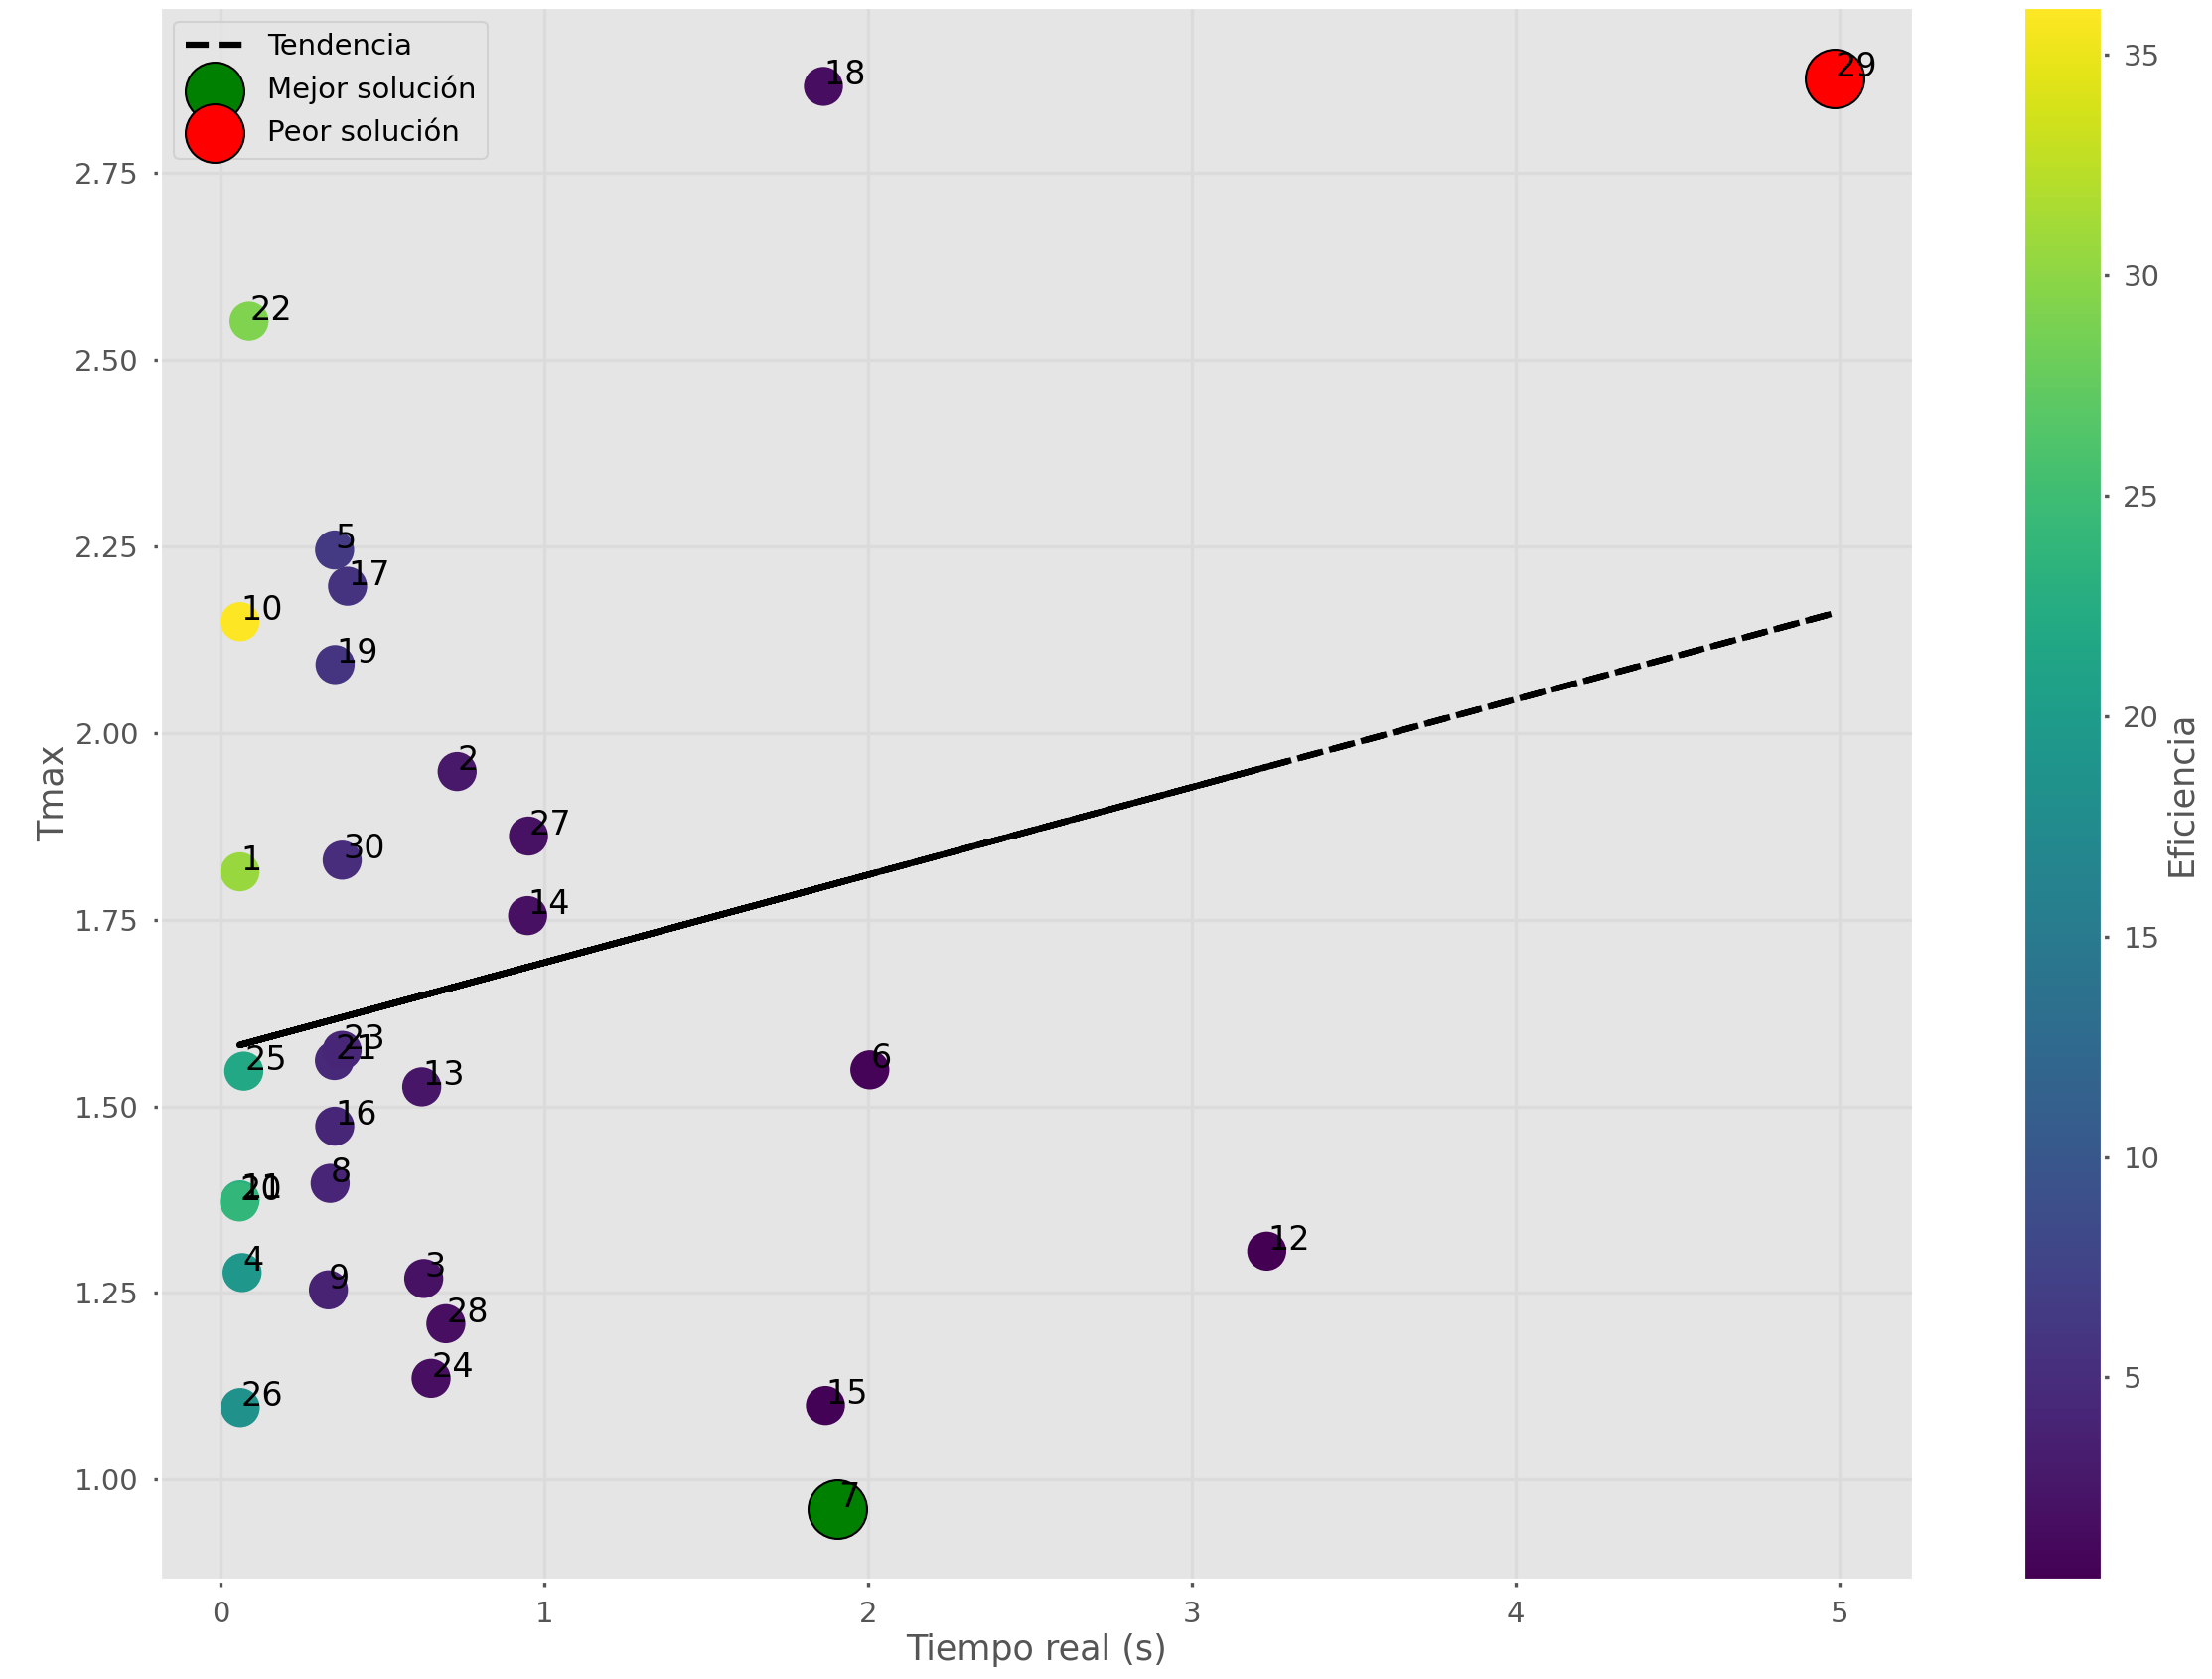
\includegraphics[scale=0.13]{Images/tema2/scatter_plot_propuesto.png}
  \caption{Diagrama de dispersión propuesto para la evaluación de la eficiencia de las soluciones. 
  Cada círculo representa una solución cuyo número adjunto corresponde con el número de ejecución, 
  el color de las soluciones se refiere a la eficiencia de las mismas, los círculos con borde negro
  representan las peor y mejor solución, en color rojo y verde, respectivamente, y la recta punteada 
  la línea de tendencia.}
  \label{fig:scatterPlot}
\end{figure}

\begin{figure}[H]
  \centering
  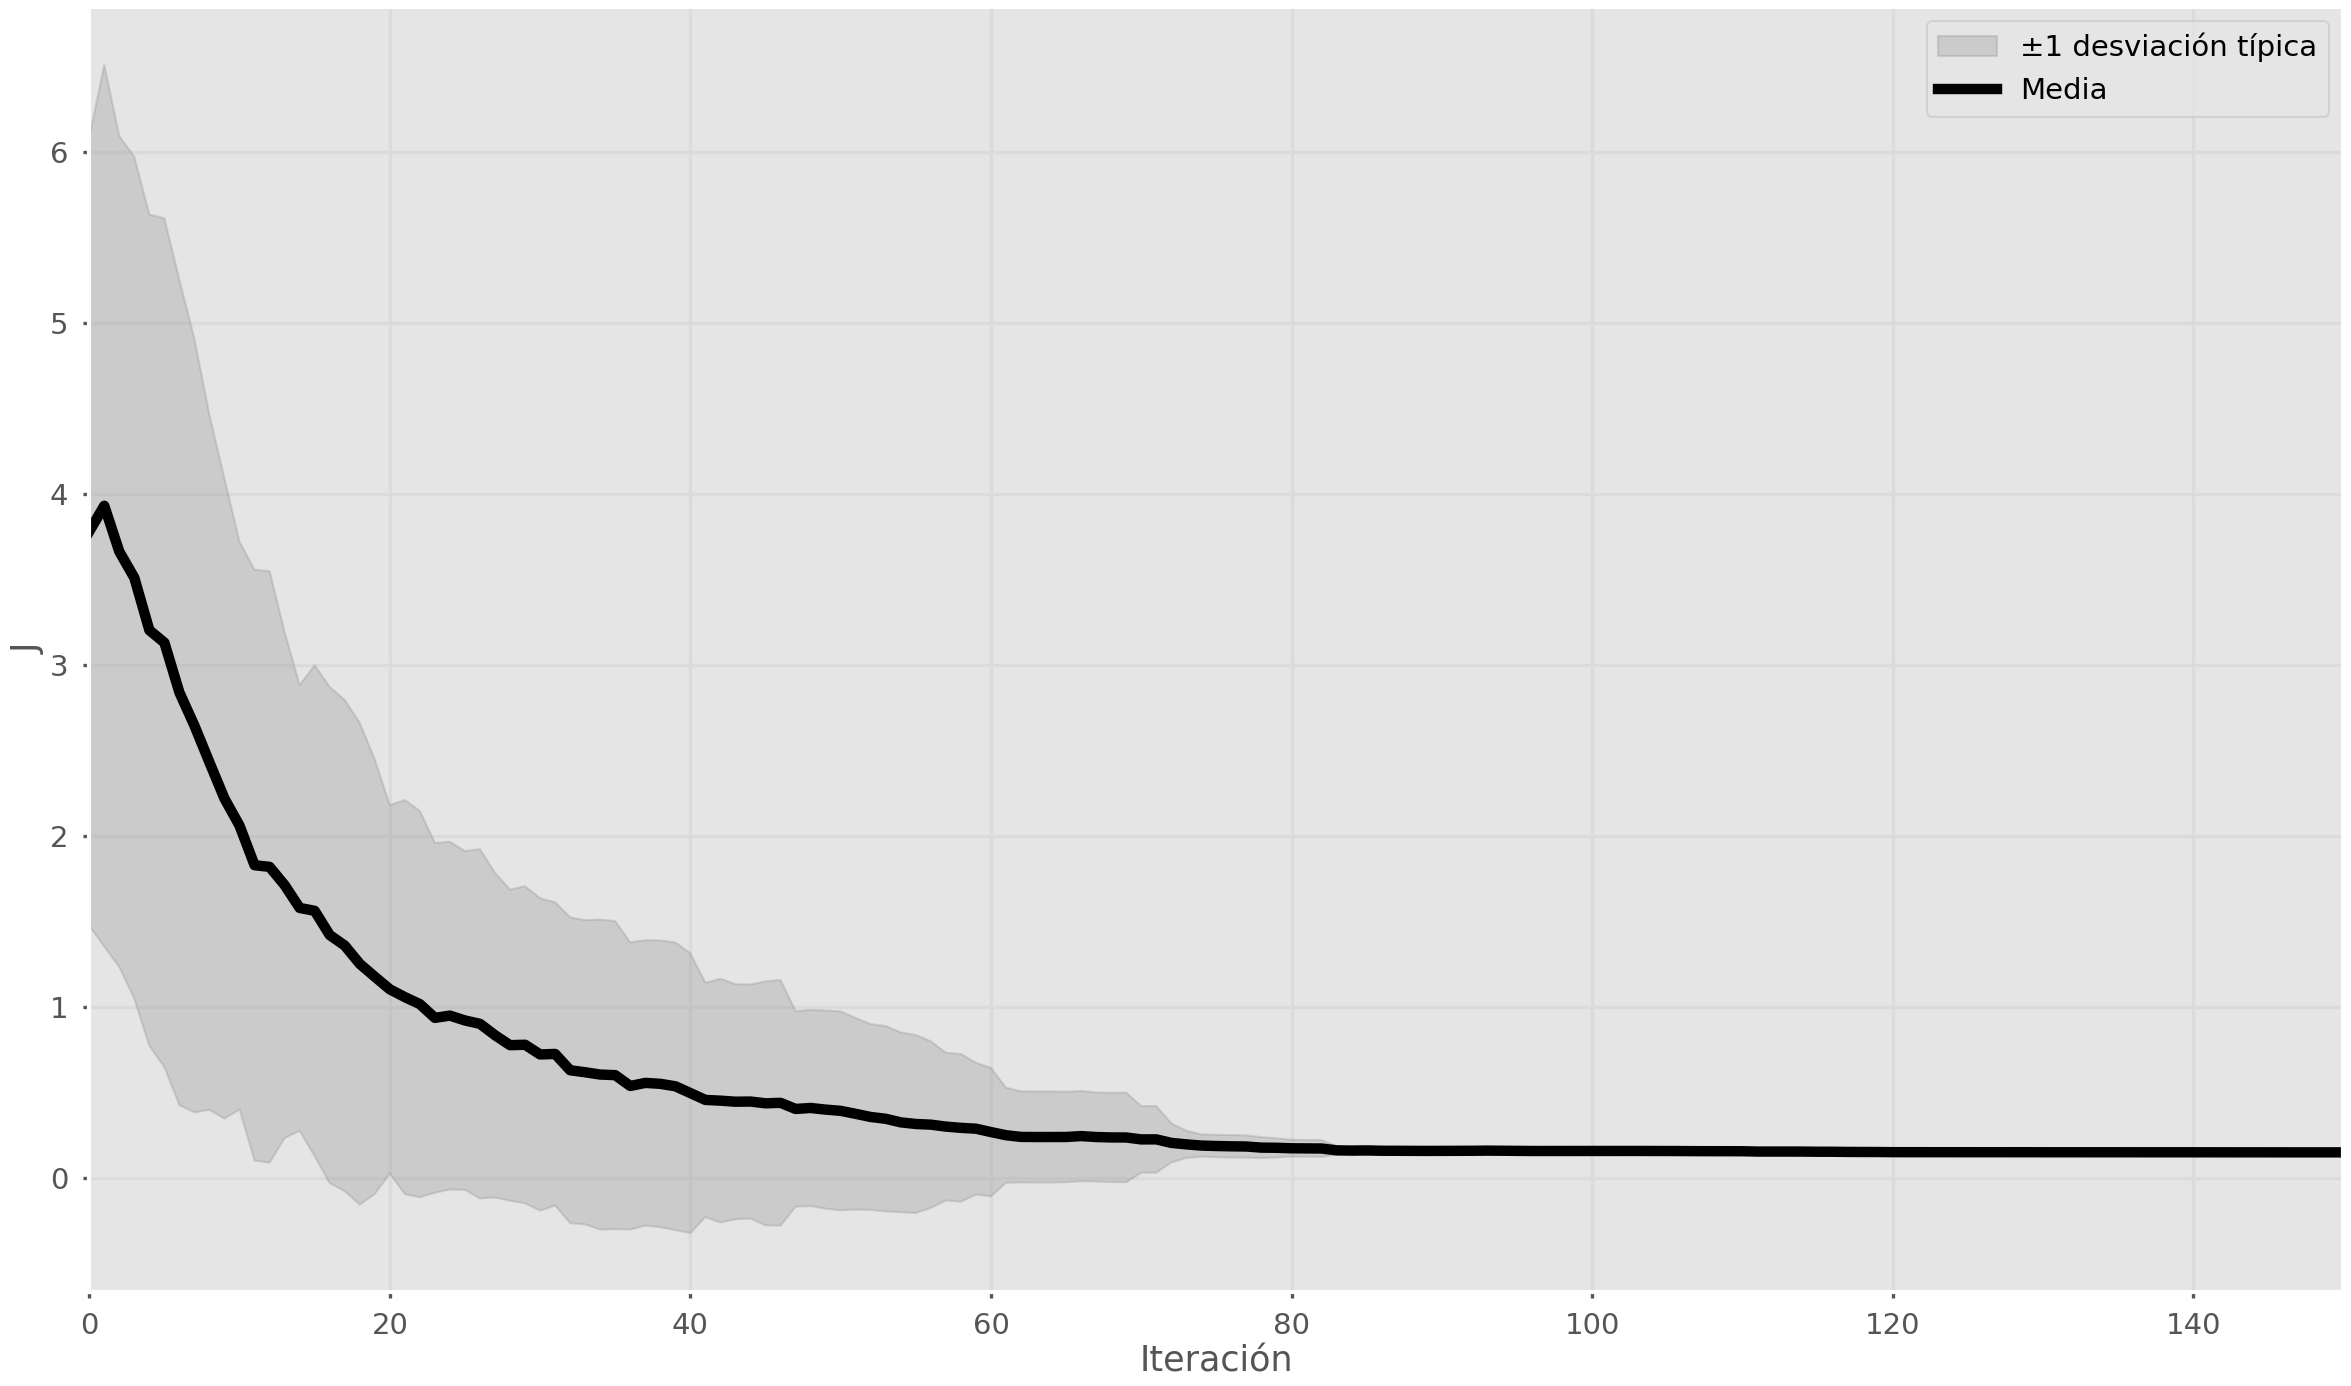
\includegraphics[scale=0.16]{Images/tema2/convergencia_media.png}
  \caption{Curva media de convergecia del método desarrollado.}
  \label{fig:curvaMedia}
\end{figure}


%En conjunto, estas métricas cuantitativas permiten concluir que el algoritmo no solo es eficaz
%en términos de calidad de las soluciones (medida mediante $T_{\max}$), sino también robusto y 
%estable en su comportamiento estadístico.


\subsection*{Conclusiones}
\addcontentsline{toc}{subsection}{Conclusiones}
Durante la evaluación de los resultados se ha observado que el algoritmo tiende a converger de forma
prematura, lo que sugiere que no está explorando completamente el espacio de soluciones
disponible. Sin embargo, las soluciones proporcionadas son muy lógicas, salvo por los perfiles 
de velocidad cuando estos reciben el máximo valor posible (1). \\

Resulta evidente que la mejor solución, es decir, aquella con menor tiempo de desplazamiento,
se obtiene con la máxima velocidad de los robots. Esta situación está introduciendo un sesgo al 
algoritmo para explorar únicamente perfiles elevados de velocidad, reduciendo el espacio de búsqueda, provocando una convergecia prematura y priorizando la minimización del tiempo a costa de ignorar
criterios de calidad del movimiento que serían relevantes en un escenario real. \\

Así todo, no todos los perfiles de velocidad optimizados son elevados, puesto que 
en la mejor solución obtenida la escala de velocidad del robot A es de $0.41$. 
Consecuentemente, demuestra que a pesar de que el algoritmo tenga un sesgo, es capaz 
de optimizar parcialmente el punto de encuentro de ambos robots. \\

La eliminación de este sesgo se plantea como línea futura, mediante la introducción
de alguna restricción sobre aceleración, suavidad o calidad de movimiento. \\

Además, el método implementado es computacionalmente eficiente puesto que 
los tiempos de ejecución son muy bajos, pudiendo ser utilizado en apliaciones de planificación 
de trayectorias de robots. \\

Por úlitmo, otro trabajo futuro que se plantea es la resolución del problema con la metodología
mencionada previamente: establecer un mecanismo de evaluación que determine cómo de lejos se 
encuentra un punto del espacio de trabajo factible para que el algoritmo de 
Temple Simulado sea capaz de converger hacia puntos factibles.

\begin{comment}

\[
p_{\text{sync}}(t_A,t_B) =
\begin{cases}
\left(\dfrac{|t_A - t_B|}{\Delta T_{\max}}\right)^2,
& \text{si } |t_A - t_B| \le \Delta T_{\max}, \

\[10pt]
1 + \left(\dfrac{|t_A - t_B| - \Delta T_{\max}}{\Delta T_{\max}}\right)^2,
& \text{si } |t_A - t_B| > \Delta T_{\max}.
\end{cases}
\]




\[
P_{\text{sing}} =
\sum_{r\in\{A,B\}}
\begin{cases}
\left(\dfrac{m_{\min} - m_r}{m_{\min}}\right)^2,
& \text{si } m_r \le m_{\min}, \

\[10pt]
0,
& \text{si } m_r > m_{\min}.
\end{cases}
\]




\[
P_{\text{sing}} =
\left(\frac{m_{\min}}{m_A}\right)^2
+
\left(\frac{m_{\min}}{m_B}\right)^2 ,
\]


% ============================================================
% DISTANCIA ARTICULAR DESDE LA POSTURA INICIAL
% ============================================================



\[
l_A = \|\, q_A - q_{A,0} \,\|
\]





\[
l_B = \|\, q_B - q_{B,0} \,\|
\]





\[
q_{A,0} = q_{B,0} = \mathbf{0}
\]





\[
l_A = \|\, q_A \,\|, 
\qquad 
l_B = \|\, q_B \,\|
\]



% ============================================================
% TIEMPO DEL ROBOT A
% ============================================================



\[
t_A = \frac{l_A}{s_A \, v_A}
\]



% ============================================================
% TIEMPO DEL RAÍL DEL ROBOT B
% ============================================================



\[
t_{\text{rail}} 
= 
\frac{\left|\, p_{\text{Rail}} - p_{\text{Rail,start}} \,\right|}
       {s_{\text{Rail}} \, v_{\text{Rail}}}
\]



% ============================================================
% TIEMPO DEL BRAZO DEL ROBOT B
% ============================================================



\[
t_{B,\text{arm}} 
= 
\frac{l_B}{s_B \, v_B}
\]



% ============================================================
% TIEMPO TOTAL DEL ROBOT B
% ============================================================



\[
t_B 
= 
t_{\text{rail}} + t_{B,\text{arm}}
\]



% ============================================================
% TIEMPO MÁXIMO (CRITERIO DE SINCRONIZACIÓN)
% ============================================================



\[
T_{\max} = \max(t_A,\, t_B)
\]



% ============================================================
% PENALIZACIÓN DE SINCRONIZACIÓN (VERSIÓN SUAVE)
% ============================================================



\[
P_{\text{sync}} =
\begin{cases}
\left(\dfrac{|t_A - t_B|}{\Delta_{\max}}\right)^2,
& |t_A - t_B| \le \Delta_{\max}
\

\[10pt]
1 + \left(\dfrac{|t_A - t_B| - \Delta_{\max}}{\Delta_{\max}}\right)^2,
& |t_A - t_B| > \Delta_{\max}
\end{cases}
\]


La temperatura inicial \(T_0\) no se ha fijado de forma arbitraria, sino a partir
de la escala observada de la función de mérito \(J\) en las primeras iteraciones.

En una fase de calibración previa, se generaron soluciones vecinas aleatorias
a partir de varias soluciones iniciales y se midieron los incrementos de coste
\(\Delta J = J_{\text{nuevo}} - J_{\text{actual}}\) para aquellos vecinos
peores que la solución actual. En nuestro problema, los valores típicos de
\(\Delta J\) en las primeras iteraciones se situaban aproximadamente en el rango
\([0.05, 0.5]\), con un valor medio alrededor de \(\overline{\Delta J} \approx 0.2\).

En Temple Simulado, la probabilidad de aceptar un empeoramiento de coste
\(\Delta J > 0\) viene dada por:



\[
P_{\text{aceptar}}(\Delta J) = \exp\left(-\frac{\Delta J}{T}\right).
\]



Si se desea una tasa de aceptación inicial alta para empeoramientos, por ejemplo
\(P_{\text{aceptar}} \approx 0.8\) para un empeoramiento típico \(\overline{\Delta J}\),
puede estimarse la temperatura inicial como:



\[
T_0 \approx -\frac{\overline{\Delta J}}{\ln(p_0)},
\qquad
p_0 \in [0.8, 0.9].
\]



Sustituyendo \(\overline{\Delta J} \approx 0.2\) y \(p_0 = 0.8\), se obtiene:



\[
T_0 \approx -\frac{0.2}{\ln(0.8)} \approx 0.9.
\]



Por simplicidad y robustez numérica se ha redondeado este valor a \(T_0 = 1\),
lo que garantiza una probabilidad de aceptación inicial elevada (del orden del
80--90\% para los empeoramientos típicos observados) y evita que el algoritmo
degenere en una búsqueda puramente ávida (Hill Climbing) en las primeras fases
de la exploración.


Aunque en la formulación general se menciona una desviación típica genérica
\(\sigma\), en la implementación práctica se ha tenido en cuenta que las
distintas variables del problema operan en escalas muy diferentes:

- Posiciones cartesianas \(p\): del orden de metros.
- Factores de velocidad \(s \in [0,1]\).
- Posición del raíl \(p_{\text{Rail}} \in [0,0.7]\).

Para evitar hiper-mutar unas variables y dejar prácticamente inalteradas otras,
se han definido desviaciones típicas específicas por tipo de variable:



\[
\sigma_p,\quad \sigma_s,\quad \sigma_{\text{rail}}.
\]



En el Nivel 1 (generación de puntos geométricos), las posiciones se generan
directamente dentro del workspace factible, por lo que no se aplica una
mutación gaussiana sobre \(p\), sino un muestreo uniforme restringido por la
geometría y la cinemática (IK + manipulabilidad). En el Nivel 2 (ajuste fino
de tiempos), las únicas variables mutadas son los factores de velocidad y la
posición del raíl, para las cuales se han elegido desviaciones típicas
específicas:



\[
s_A, s_B, s_{\text{Rail}} \in [0,1], \qquad
\sigma_s = 0.05,
\]





\[
p_{\text{Rail}} \in [0,0.7], \qquad
\sigma_{\text{rail}} = 0.05.
\]



Estas desviaciones se han sintonizado empíricamente para que:

1) La mayoría de las mutaciones produzcan cambios apreciables en el coste
   (evitando pasos demasiado pequeños que no exploran el espacio), y

2) Una fracción significativa de vecinos siga siendo aceptable, de modo que
   el Temple Simulado mantenga un buen equilibrio entre exploración y
   explotación.

En resumen, aunque en la descripción teórica se menciona una \(\sigma\) única,
en la implementación se ha respetado la escala de cada tipo de variable mediante
parámetros \(\sigma\) diferenciados, lo que evita desbalances entre la mutación
de posiciones, velocidades y raíl.


En código, esto se refleja en:

\begin{verbatim}
new.sA = np.clip(new.sA + np.random.normal(0, sigma_s), 0.0, 1.0)
new.sB = np.clip(new.sB + np.random.normal(0, sigma_s), 0.0, 1.0)
new.sRail = np.clip(new.sRail + np.random.normal(0, sigma_s), 0.0, 1.0)

new.pRail += np.random.normal(0, sigma_prail)
new.pRail = np.clip(new.pRail, new.rail_min, new.rail_max)
\end{verbatim}
\end{comment}
%\include{propuesta2}
%\include{propuesta3}

\newpage
\datos{color}{}{}
\printbibliography[title={Referencias adicionales al Campus Virtual}]
\addcontentsline{toc}{section}{Referencias adicionales al Campus Virtual}

\end{document}
